\documentclass[xcolor=pdftex,dvipsnames,table]{beamer}
\usepackage{import}

\usepackage{enumerate}
%\usepackage[table]{xcolor}
\usepackage{graphics}
\usepackage{graphicx}
\usepackage{mathrsfs}
\usepackage{multirow}
\usepackage{hhline}
\usepackage{pbox}
\usepackage{hyperref}
%\usepackage[backend=bibtex,style=authoryear,natbib=true]{biblatex} % Use the bibtex backend 
\usepackage[scaled]{helvet}
\usepackage[round]{natbib}
%\newcommand{\newblock}{}

\usepackage{fancyhdr}
\usepackage{amsmath,amssymb,amsthm,esint}
\usepackage{longtable}
\usepackage{tikz}
\usepackage{float}
\usepackage{pgfplots}
\usepackage{caption}
\usepackage{subcaption}
\usepackage{empheq}
\usepackage{indentfirst}
\usepackage{algorithm}
\usepackage{algpseudocode}

\usepackage[many]{tcolorbox}
\usepackage[T1]{fontenc}
\usepackage[utf8]{inputenc}
%\usepackage{lmodern}
\usepackage[english]{babel}
\newcommand{\wto}{\rightharpoonup}

\usepackage{makeidx}

%\newtheorem{theorem}{Theorem}[section] 
\newtheorem{acknowledgement}[theorem]{Acknowledgement}
%\newtheorem{algorithm}[theorem]{Algorithm}
\newtheorem{axiom}[theorem]{Axiom}
\newtheorem{case}[theorem]{Case}
\newtheorem{claim}[theorem]{Claim}
\newtheorem{conclusion}[theorem]{Conclusion}
\newtheorem{condition}[theorem]{Condition}
\newtheorem{conjecture}[theorem]{Conjecture}
%\newtheorem{corollary}[theorem]{Corollary}
\newtheorem{criterion}[theorem]{Criterion}
\newtheorem{conditions}[theorem]{Conditions}
%\newtheorem{definition}[theorem]{Definition}
%\newtheorem{example}[theorem]{Example}
\newtheorem{exercise}{Exercise}
%\newtheorem{lemma}[theorem]{Lemma}
\DeclareMathOperator*{\argmax}{arg\,max}
\DeclareMathOperator*{\argmin}{arg\,min}
\DeclarePairedDelimiter{\ceil}{\lceil}{\rceil}
\DeclarePairedDelimiter\floor{\lfloor}{\rfloor}
%%%%%%%%%%%%%%%% My Commands/Shorthand %%%%%%%%%%%%%%%%
%\newcommand{\qed}{\hfill\ensuremath{\Box}}
\newcommand{\qedb}{\hfill \blacksquare}
\newcommand{\wrt}{w.r.t}
\newcommand{\rml}{\multicolumn{1}{c}{}}
\newcommand{\tbf}[1]{\textbf{#1}}
\newcommand{\ib}[1]{\item \textbf{#1}}
\newcommand{\B}{\mathcal{B}}
\newcommand{\R}{\mathbb{R}}
\newcommand{\re}{\text{Re}}
%\newcommand{\Z}{\mathbb{Z}}
\newcommand{\TT}{\mathbb{T}}
\newcommand{\T}{\mathcal{T}}
%\newcommand{\S}{\mathcal{S}}
\newcommand{\N}{\mathbb{N}}
\newcommand{\X}{\mathcal{X}}
\newcommand{\M}{\mathcal{M}}
\newcommand{\MO}{\mathcal{O}}
\newcommand{\prob}{\text{Prob}}
\newcommand{\var}{\text{Var}}
\newcommand{\Q}{\mathbb{Q}}
\newcommand{\C}{\mathbb{C}}
\newcommand{\CC}{\mathcal{C}}
\newcommand{\fl}{\text{fl}}
\newcommand{\sign}{\text{sign}}
\newcommand{\relu}{\text{ReLU}}
\newcommand{\norm}[1]{\left\lvert #1 \right\rvert}
\newcommand{\Norm}[1]{\left\lVert #1 \right\rVert}
\newcommand{\ip}[1]{\left\langle #1 \right\rangle}
\def\tesst{https://chrome.google.com/webstore/detail/slack-bot-filter/blephhkggdennbfmdcjmlfimedknghfc}
\def\lvector#1{\underline{#1}}
\def\lmatrix#1{\underline{\underline{#1}}}
\def\ltensor#1{\underline{\underline{\underline{#1}}}}
\DeclareMathOperator\vol{\text{vol}}
\newcommand{\e}{\varepsilon}

%\usepackage{mathabx}


%%%%%%%%%%%%%%%% TIKZ stuff %%%%%%%%%%%%%%%%
    \pgfplotsset{compat=newest}
    \usetikzlibrary{shapes,arrows,matrix,positioning,intersections}
    \usetikzlibrary{calc}
%    \usetikzlibrary{decorations.pathreplacing}
    \usetikzlibrary{decorations} %fancier tikz abilities
    \pgfdeclarelayer{bg}
    \pgfsetlayers{bg,main}
		% Define block styles
    \tikzstyle{decision} = [diamond, draw, fill=blue!20, 
        text width=3cm, text badly centered, node distance=3cm, inner sep=0pt]
    \tikzstyle{block} = [rectangle, draw, fill=blue!20, 
        text width=3cm, text centered, rounded corners, minimum height=2em]
    \tikzstyle{line} = [draw, -latex']
    \tikzstyle{cloud} = [draw, ellipse,fill=red!20, node distance=3cm,
        minimum height=2em]

\usetikzlibrary{decorations.text,arrows.meta}
\usetikzlibrary{decorations.pathmorphing}
\usetikzlibrary{decorations.markings} %hopefully give arrows

\tikzset{
  % style to apply some styles to each segment of a path
  on each segment/.style={
    decorate,
    decoration={
      show path construction,
      moveto code={},
      lineto code={
        \path [#1]
        (\tikzinputsegmentfirst) -- (\tikzinputsegmentlast);
      },
      curveto code={
        \path [#1] (\tikzinputsegmentfirst)
        .. controls
        (\tikzinputsegmentsupporta) and (\tikzinputsegmentsupportb)
        ..
        (\tikzinputsegmentlast);
      },
      closepath code={
        \path [#1]
        (\tikzinputsegmentfirst) -- (\tikzinputsegmentlast);
      },
    },
  },
  % style to add an arrow in the middle of a path
  mid arrow/.style={postaction={decorate,decoration={
        markings,
        mark=at position .5 with {\arrow[#1]{stealth}}
      }}},
}

%%%%%%%%%%%%%%%% Table of Contents Stuff %%%%%%%%%%%%%%%%
\setcounter{secnumdepth}{3} % if set to -1 only chapter and sections will be numbered
\setcounter{tocdepth}{4}

%%%%%%%%%%%%%%%% Hyper Ref Stuff %%%%%%%%%%%%%%%%
		% set up reference style
\hypersetup{
    linktoc=all,		% build toc with internal links
    unicode=false,         	% non-Latin chars in Acrobat bookmarks
    pdftoolbar=true,       	% show Acrobats toolbar?
    pdfmenubar=true,       	% show Acrobats menu?
    pdffitwindow=false,    	% window fit to page when opened
    pdfstartview={FitH},   	% fits width of page to the window
    pdftitle={My title},   	% title
    pdfauthor={Author},    	% author
    pdfsubject={Subject},  	% subject of the document
    pdfcreator={Creator},  	% creator of the document
    pdfproducer={Producer},	% producer of the document
    pdfkeywords={keyword1} {key2} {key3}, % list of keywords
    pdfnewwindow=true,      	% links in new window
    colorlinks=true,       	% false: boxed links; true: colore links
    linkcolor=blue,          	% color of internal links (change box
				% color with linkbordercolor)
    citecolor=green,        	% color of links to bibliography
    filecolor=magenta,      	% color of file links
    urlcolor=cyan           	% color of external links
}

%%%%%%%%%%%%%%%% My Commands/Shorthand %%%%%%%%%%%%%%%%
% \newcommand{\qed}{\hfill\ensuremath{\Box}}

% \newcommand{\qedb}{\hfill \blacksquare}
% \newcommand{\LIM}{\text{LIM}}
% \newcommand{\wrt}{w.r.t}
% \newcommand{\rml}{\multicolumn{1}{c}{}}
% \newcommand{\tbf}[1]{\textbf{#1}}
% \newcommand{\ib}[1]{\item \textbf{#1}}
% \newcommand{\B}{\mathcal{B}}
%\newcommand{\R}{\mathbb{R}}

% \newcommand{\K}{\mathbb{K}}
% \newcommand{\F}{\mathbb{F}}
% \newcommand{\re}{\text{Re}}
% %\newcommand{\Z}{\mathbb{Z}}
% \newcommand{\TT}{\mathbb{T}}
% \newcommand{\T}{\mathcal{T}}
% %\newcommand{\S}{\mathcal{S}}
% \newcommand{\N}{\mathbb{N}}
% \newcommand{\M}{\mathcal{M}}
% \newcommand{\MO}{\mathcal{O}}
% \newcommand{\prob}{\text{Prob}}
% \newcommand{\var}{\text{Var}}
% \newcommand{\Q}{\mathbb{Q}}
% \newcommand{\C}{\mathbb{C}}
% \newcommand{\E}{\mathcal{E}}
% \newcommand{\fl}{\text{fl}}
% \newcommand{\sign}{\text{sign}}
% \newcommand{\norm}[1]{\left\lvert #1 \right\rvert}
% \newcommand{\Norm}[1]{\left\lVert #1 \right\rVert}


% \newcommand*\circled[1]{\tikz[baseline=(char.base)]{
%             \node[shape=circle,draw,inner sep=2pt] (char) {#1};}}

% \newcommand{\nifty}{\textbf{NIFTY}}




\tcbset{breakable,
skin=bicolor,
colback=black!15!white,
colbacklower=white,
colframe=black!25!white,
coltitle=black,
fonttitle=\bfseries,
boxrule=1pt,
boxsep=3.0pt,
left=0.0pt,
right=0.0pt,
top=0.0pt,
bottom=0.0pt,
middle = 1.0pt,
arc = 0.0pt,
outer arc = 0.0pt,
frame style={top color=white,
bottom color=white,draw=black},
interior style={left color=black!0!white,right color=black!0!white},
segmentation style={right color=white,left color=white}
}

\DeclareMathOperator{\Tr}{Tr}


\author{Brian Bell : University of Arizona}
\date{\today}
\title{A Geometric Framework for Adversarial Vulnerability in
  Machine Learning}

\def\layersep{2.0cm}


%\documentclass{beamer}

\mode<presentation>
{
  \usetheme{Boadilla}
  % possiblities Singapore, Malmoe, Dresden 
  %\setbeamercovered{transparent}
}

 
%\setbeamertemplate{navigation symbols}{} 
% removes the navigation symbols

%color setting more or less matching U of A colors
\setbeamercolor*{palette secondary}{use=structure,fg=white,bg=structure.fg!55!black}
\setbeamercolor*{palette tertiary}{use=structure,fg=white,bg=red!50!black}



\setbeamertemplate{bibliography item}{\insertbiblabel}

\setbeamertemplate{background}{
\tikz[overlay,remember picture]
\node[opacity=0.02,anchor=south east, fill=white, inner sep=10pt] (a) at (current
       page.south
       east){
\includegraphics[width=.5in,]{university_of_arizona-eps-converted-to.pdf}};  }
% \fill[width=1in, white] (a.south west) rectangle (a.north east);}



% Delete this, if you do not want the table of contents to pop up at
% the beginning of each section:
\AtBeginSection[]
{
  \begin{frame}<beamer>
    \frametitle{Contents}
    {
    \tableofcontents[currentsection]
        }
  \end{frame}
}

% If you wish to uncover everything in a step-wise fashion, uncomment
% the following command: 
%\beamerdefaultoverlayspecification{<+->}
\defbeamertemplate*{title page}{customized}[1][]
{
  \centering
  \usebeamerfont{title}\usebeamercolor[fg]{title}\Large\inserttitle\par
  \usebeamerfont{subtitle}\usebeamercolor[fg]{subtitle}\insertsubtitle\par
  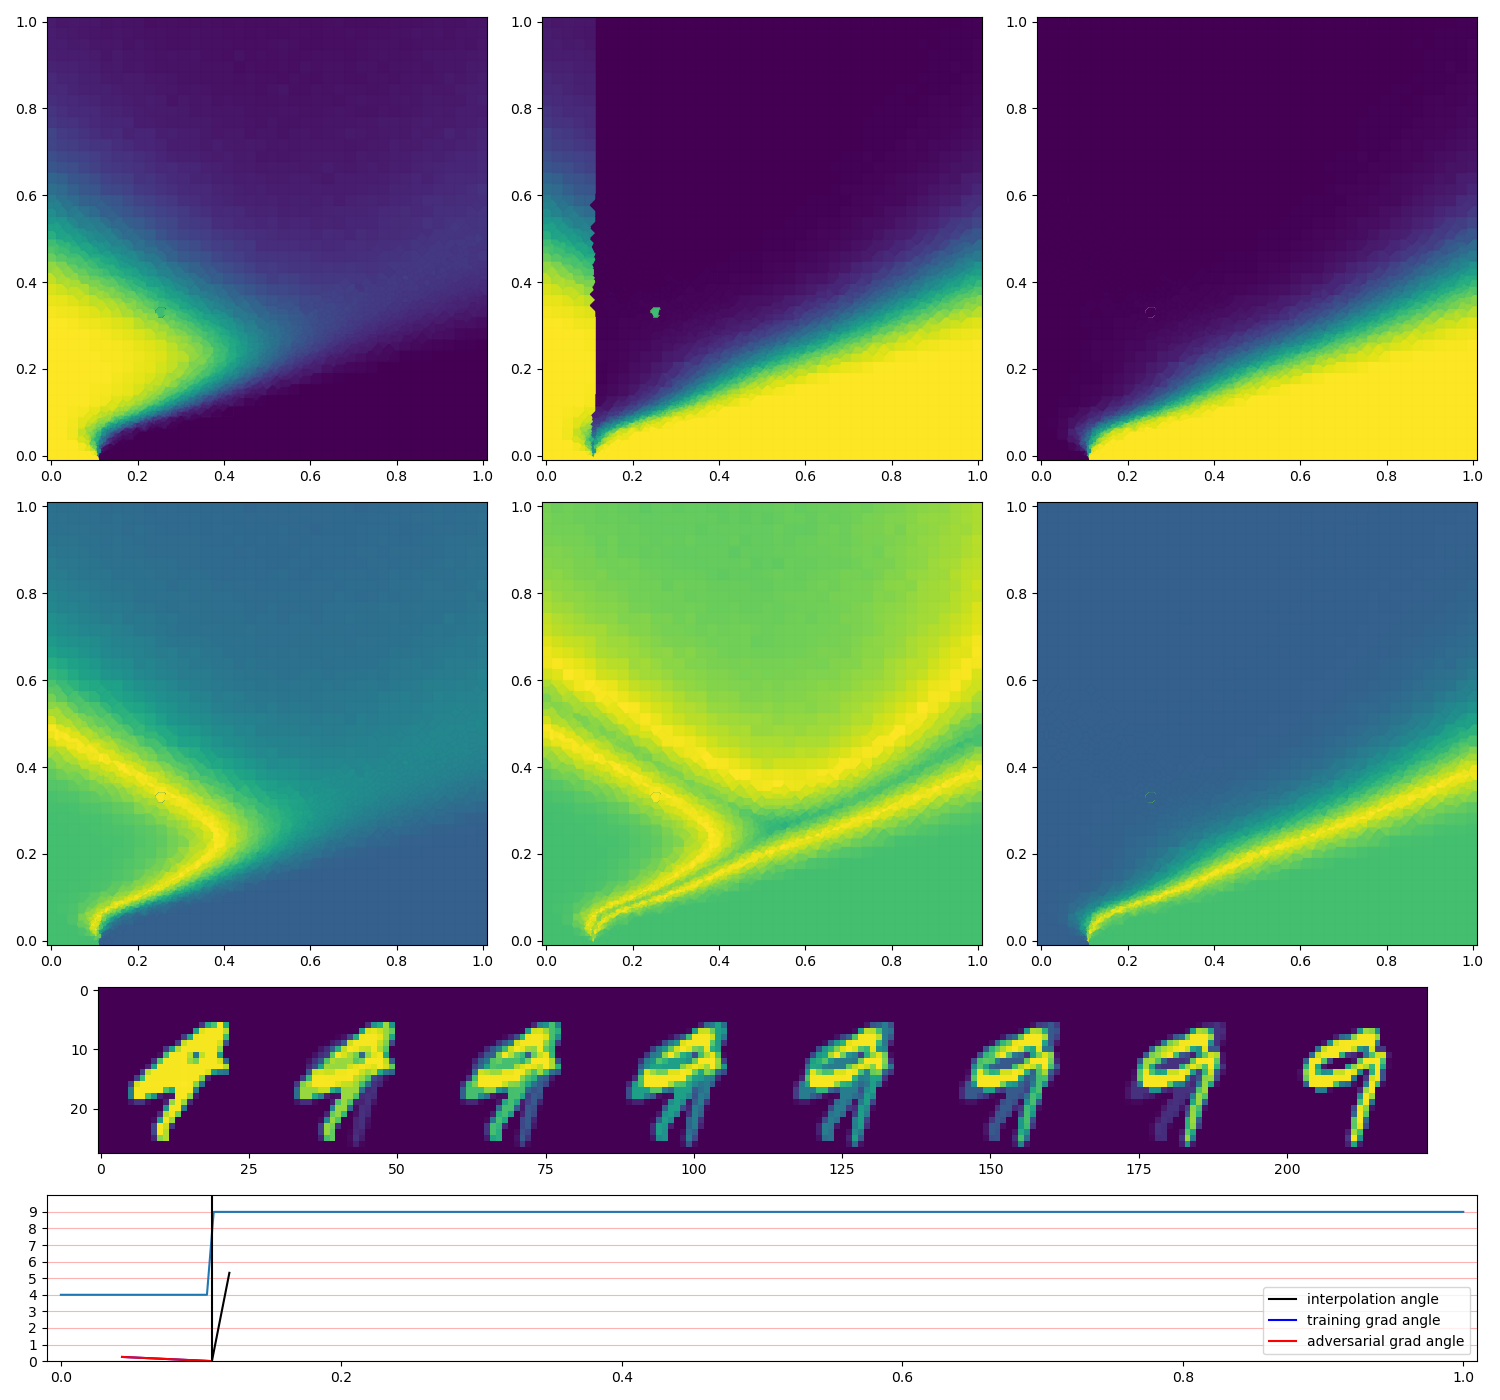
\includegraphics[width=0.42\textwidth]{stab-mnist-C32-50-50-10-0.001-eval-1e-06-none-4-9-db_interp-stability-51.png}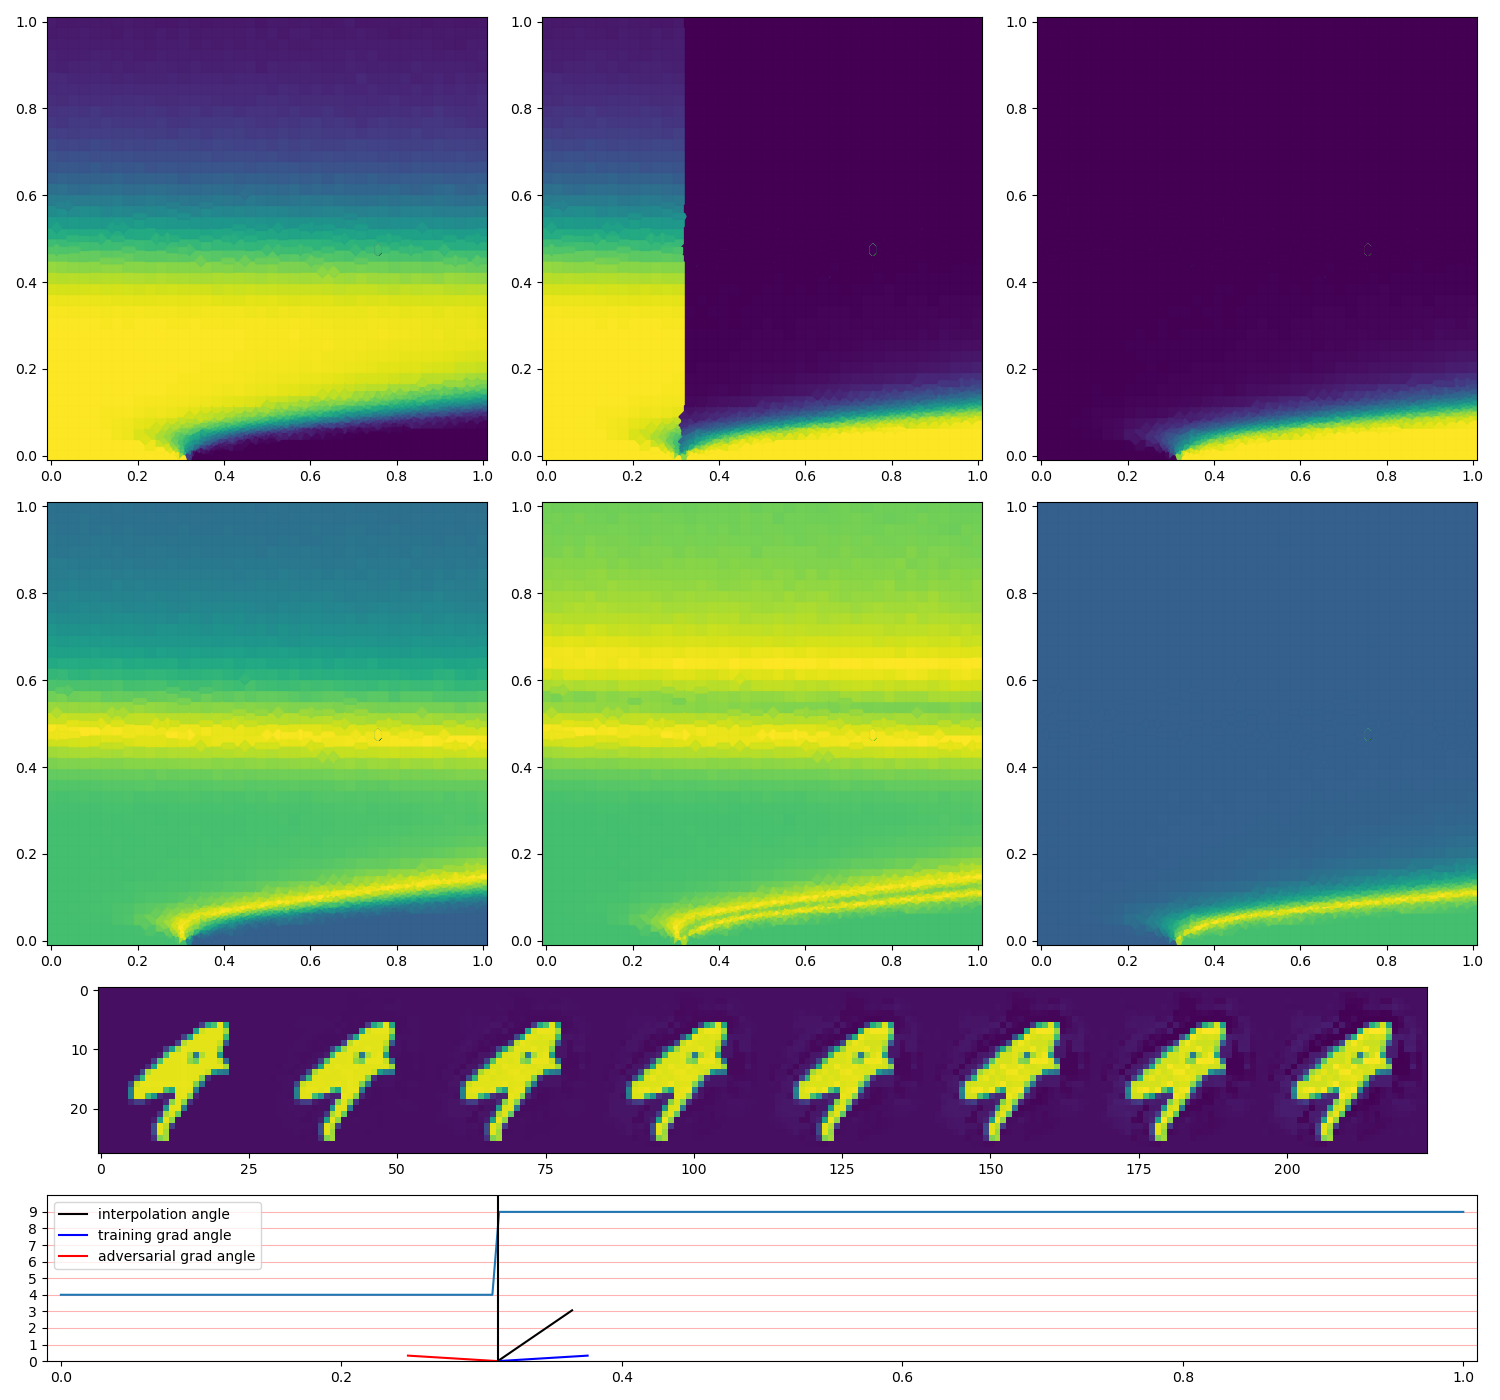
\includegraphics[width=0.42\textwidth]{stab-mnist-C32-50-50-10-0.001-eval-1e-06-pgd-4-9-db_interp-stability-51.png} 
  
  \usebeamerfont{author}\usebeamercolor[fg]{black}\insertauthor\par
  \usebeamerfont{institute}\insertinstitute\par
  \usebeamerfont{date}\normalsize\insertdate\par
  \usebeamercolor[fg]{titlegraphic}\inserttitlegraphic
}


\begin{document}

\begin{frame}
  \titlepage
\centering

\end{frame}

% Introduction
% historical timeline
% reference some explanatory pictures
% introduce some notation
% main takeaways the mathematical elements are simple but notation is
%a limitation.
%% Introduction
% historical timeline
% reference some explanatory pictures
% introduce some notation
% main takeaways the mathematical elements are simple but notation is
%a limitation.
\part{Introduction} % Main chapter title
\label{Chapter1} % For referencing the chapter elsewhere, use \ref{Chapter1} 

% \begin{frame}[fragile]
% \frametitle{Neural Network}

% \scalebox{.9}{
% \begin{frame}[fragile]
% \frametitle{Neural Network}

% \scalebox{.9}{
% }
% \end{frame}

%%%%%%%%%%%%%%%%%%%%%%%%%%%%%%%%%%%%%%%%%(1)
\begin{frame}
  \frametitle{Goals}
  \begin{itemize}
      % \item<1-> Describe brief history of machine-learning. 
      \item<1-> Understand (mathematically) what Artificial Neural
        Networks (ANNs) are and how they are being used. 
      \item<2-> Define a geometric approach to interpreting neural
        network classifiers. 
      \item<3-> Connect geometric approach with concept of 
        robustness. 
      \item<4-> Define a kernel based representation which allows application
        of kernel based tools to ANNs
      \item<5-> Leverage our kernel based representation and these
        tools to get some useful results!
      \item<6-> Lay out further work which will connect representation
        approach to the geometric properties observed earlier. 
  \end{itemize}
\end{frame}

% transition from task specific models to foundation models --
% Models are starting to have a "general" geometric understanding of
% the data. 
\section{Background}

\begin{frame}
  \frametitle{History : Beginnings in Theory of Cognition}
  \begin{itemize}
     \item<1->  The mechanics of cognition are described in the context of
      computation by ~\citet{mcculloch1943logical}. 
      \item<2-> The perceptron $f(x) = A(w \cdot x + b)$, the
        most granular element of a neural network, is proposed by
        ~\citet{rosenblatt1958perceptron}. 
      \item<3->  Perceptrons are assembled into multilevel (deep)
        networks ($A_n \circ f_n \circ
        \cdots \circ f_3 \circ A_2 \circ f_2 \circ
        A_1 \cdots f_1$) by ~\citet{ivakhnenko1965cybernetic}
      \item<5->  ~\citet{minsky1969perceptrons} present a proof that
        basic perceptrons could not encode exclusive-or. 
      \item<6->  Neural Networks become disassociated from Cognitive
        Science and Computational Limitations curtail industrial
        applications. 
      \item<7-> Interest in Neural Networks wanes. 
  \end{itemize}
\end{frame}

\begin{frame}
  \frametitle{History : Revolution}
  \begin{itemize}
      \item<1-> ~\citet{linnainmaa1970representation} proposes
        a computation for gradients of large-scale multi-parameter
 models in his masters thesis. Back-Propagation is born!
      \item<2->  A Harvard student,  ~\citep{werbos1974beyond},
        applies this technique to ANNs. 
      \item<3->  ~\citet{mcclelland1986parallel} propose distributed
        processing in the context of cognition allowing tree-like
        computations to be processed in separate computing threads. 
      \item<4-> Finally, these pieces are brought together by
        ~\citet{lecun1989backpropagation}. 
      \item<5->  ~\citep{lecun1995convolutional} invent convolutional
        neural networks which are more capable and scale more
        cheaply.
        \item <6-> This completed tools is applied to the
        lucrative task of handwriting recognition
        ~\citep{lecun1998gradient} and the commercial viability of
        ANNs is established. 

  \end{itemize}
\end{frame}

\begin{frame}
  \frametitle{History : Explosion}
  \begin{itemize}
     \item<1-> Neural Networks' industrial success fuels a new wave of
       serious research and development including the now famous
       PyTorch ~\citep{Collobert2002TorchAM} 
       
     \item<2-> Geoffrey Hinton is among the first to comprehensively understand
       how to scale ``deep'' learning models
       ~\citep{hinton2006reducing, hinton2006fast} along with Samy
       Bengio ~\citep{bengio2009learning}. 

       % \item<3-> Recurrent networks, applying  earlier work on
       %   Long-Short-Term-Memory (LSTM) networks
       %   ~\citep{hochreiter1997long} to overcome vanishing gradients, are implemented
       %   ~\citep{mikolov2010recurrent}. 

       \item<3-> Recurrent ANNs are applied to natural
language processing ~\citep{collobert2011natural}
       \item<4-> ~\citet{szegedy2013} discover easily scalable
         adversarial attacks against neural networks!

      \item<5-> Networks trained on Google's ImageNet database (>14M
        images, >20K categories) outperform humans on classification
        tasks \citep{SCHMIDHUBER201585}
      \visible<4>{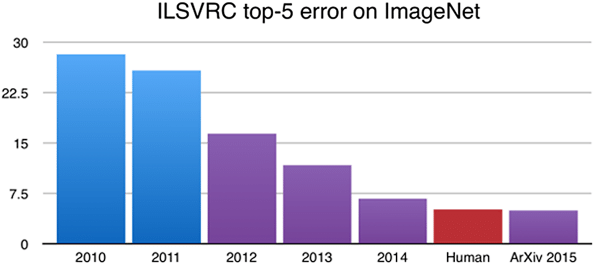
\includegraphics[width=7cm]{imnet_progress.png}}
  \end{itemize}
\end{frame}


\subsection{Structure}
% In this subsection we give a mathematical description of artificial neural networks. 

% %TODO: change this definition to something very vague and general -- use wikipedia 
% \begin{definition}{A \textbf{Neuron} is  }
%    a nonlinear operator that takes input in $\R^n$ to $\R$, historically designed to emulate the activation characteristics of an organic neuron.
%    \end{definition}

% \begin{frame}
%   \frametitle{Definitions : ANN}
% \begin{definition}{A \textbf{Neuron} is  } a nonlinear operator that
%   takes input in $\R^n$ to $\R$, historically designed to emulate the
%   activation characteristics of an organic neuron. A collection of
%   neurons that are connected via a (usually directed) graph structure
%   are known as an \emph{Artificial Neural Network (ANN)}.
% \end{definition}


% \end{frame}
\begin{frame}
  \frametitle{Definitions : Building Blocks}

The fundamental building blocks of most ANNs are artificial neurons which we will refer to as \emph{perceptrons}.

\begin{definition}{A \textbf{Perceptron} is  }
\label{perceptron}
a function $P_{\vec w}: \R^n \to \R$ which has \emph{weights} $\vec
w \in \R^n$ corresponding with each element of an input vector $\vec
x\in \R^n$ and a bias $b \in \R$:
\[P_{\vec w}(\vec x) = f(\left(\ip{\vec w,\vec x} + b\right)\]
\[P_{\vec w}(\vec x) = f\left(b + \sum_{i = 1}^n w_i x_i\right)\]
where $f: \R \to \R$ is continuous. The function $f$ is called the \textbf{activation function} for $P$. 
\end{definition}

\end{frame}

\begin{frame}
  \frametitle{Definitions : Perceptron}
  Perceptrons have a few notable properties
  \begin{itemize}
  \item $w \cdot x + b$ is linear.
    \item The activation function $f$ must contain all non-linearity
      needed for universal function approximation.
      \item In order to approximate arbitrary nonlinear functions, $f$ must
        not be linear ~\citep{attali1997approximations}.
        \item Arbitrarily many perceptrons can be connected in a
          tree-structure.
\end{itemize}
\end{frame}
      

\begin{frame}
 \frametitle{Definitions : ReLU}
\begin{definition}{The Rectified Linear Unit (ReLU) function is}
\label{relu}
   \[\relu(x) = \begin{cases} 0, & x \leq 0;\\
       x, & x > 0,\end{cases}\]
 \end{definition}

\begin{itemize}
    \item ~\citet{glorot2011deep} showed that
      Rectified Linear Units (ReLU) can out-perform smoother
      activation functions e.g. sigmoids.
    \item ReLU Networks even converge faster according to
      ~\citet{nair_rectified_nodate}!
    \item  ~\citet{petersen2018optimal} demonstrated that this single
      nonlinearity of this activation function
at $x = 0$ is sufficient to guarantee existence of $\epsilon$ approximation of smooth functions
\end{itemize}
\end{frame}





% In general ANNs 
% must not be cyclic and, for convenience, are often arranged into
% independent layers. An early roadblock for neural networks was a proof
% by ~\citet{minsky1969perceptrons} that single layers of perceptrons
% could not encode exclusive-or. ~\citet{kak1993training} demonstrated
% that depth, the number of layers in a neural network, is a key factor in its ability to approximate complicated functions including exclusive-or . For this reason, modern ANNs are usually composed of many layers (3-100). The most common instance of a neural network model is a fully connected \emph{feed forward (FF)} configuration. In this configuration data enters as an input layer which is fed into each of the nodes in the first layer of neurons. Output of the first layer is fed into each of the nodes in the second layer, and so on until the output of the final layer is fed into an output filter which generates the final result of the neural network. 



\begin{frame}
  \frametitle{Example : Fully Connected Feed Forward Network}
% In this example of a FF network, an input vector in $\R^7$ is mapped to a
% an output in $\R^3$ which is fed into a classifier. Each blue circle
% represents a perceptron with the ReLU activation function. 
\centering
\scalebox{.9}{
\begin{tikzpicture}[shorten >=1pt,->,draw=black!50, node distance=\layersep]
    \tikzstyle{every pin edge}=[<-,shorten <=1pt]
    \tikzstyle{neuron}=[circle,fill=black!25,minimum size=9pt,inner sep=0pt]
    \tikzstyle{input neuron}=[neuron, fill=green!50];
    \tikzstyle{output neuron}=[neuron, fill=red!50];
    \tikzstyle{hidden neuron}=[neuron, fill=blue!50];
    \tikzstyle{annot} = [text width=4em, text centered]

    % Draw the input layer nodes
    \foreach \name / \y in {1,...,7}
    % This is the same as writing \foreach \name / \y in {1/1,2/2,3/3,4/4}
        \node[input neuron] (I-\name) at (0,-\y) {};
%pin=left:Input \#\y
    % Draw the hidden layer nodes
    \foreach \name / \y in {1,...,6}
        \path[yshift=-0.5cm]
            node[hidden neuron] (H-\name) at (\layersep,-\y cm) {};

    \foreach \name / \y in {1,...,4}
        \path[yshift=-1.5cm,xshift=2.0cm]
            node[hidden neuron] (HH-\name) at (\layersep,-\y cm) {};

    \foreach \name / \y in {1,...,3}
        \path[yshift=-2cm,xshift=4.0cm]
            node[output neuron] (O-\name) at (\layersep,-\y cm) {};

    % Draw the output layer node
%   \foreach \name / \y in {1,...,3}
%        \path[yshift=-1.5cm,xshift=4.0cm]
%            \node[output neuron] (O-\name) at (\layersep,-\y cm) {};


    % Connect every node in the input layer with every node in the
    % hidden layer.
    \foreach \source in {1,...,7}
        \foreach \dest in {1,...,6}
            \path (I-\source) edge (H-\dest);

    \foreach \source in {1,...,6}
        \foreach \dest in {1,...,4}
            \path (H-\source) edge (HH-\dest);

    % Connect every node in the hidden layer with the output layer
    \foreach \source in {1,...,4}
        \foreach \dest in {1,...,3}
            \path (HH-\source) edge (O-\dest);

    % Annotate the layers
  \node [rectangle, draw, minimum height=6.2cm, text width=.8cm, text
  centered, left =.8cm of I-4] (mm) {Data};

    \foreach \source in {1,...,7}
        \path [line] (mm.east|-I-\source) -- (I-\source);

    \node[annot,above of=H-1, node distance=2cm] (hl) {Layer 1};
    \node[annot,left of=hl] {Input };
    \node[annot,right of=hl] (h3) {Layer 2} ;
    \node[annot,right of=h3] {Output Layer};
  \node [rectangle, draw, minimum height=5cm, text width=1.6cm, text
  centered, right =6.8cm of I-4] (mc) {Classifier};
    \foreach \source in {1,...,3}
        \path [line] (O-\source) -- (mc.west|-O-\source);


\end{tikzpicture}
}
\end{frame}


% The output of this ANN is fed into a classifier. To complete this
% example, we can define the most common classifier, Softmax:

\begin{frame}
  \frametitle{Definition : Softmax Classifier}
\begin{definition}{Softmax (or the normalized exponential) is the function given by}
\[s : \R^n \to [0,1]^n\]
\[s_j(\vec x) = \frac{e^{x_j}}{\sum_{k = 1}^n e^{x_k}}\]
\end{definition}

\begin{definition}{We can define a classifier which picks the class corresponding with the largest output element from Softmax: }
\[\text{(Output Classification)  }   c_s(\vec x) = \text{argmax}_{i} s_i(\vec{x})\]
\end{definition}
\end{frame}

% % It is important that the classifier admit a directed error function
% During training, the output $y \in \R^n$ from a network can thus be
% compressed using softmax into $[0,1]^n$ as a surrogate for probability
% for each possible class or directly into the classes which we can
% represent as the simplex for the vertices of $[0,1]^n$
% \citep{Bishop:2006:PRM:1162264}. 

% \subsubsection{Convolutional Neural Networks (CNNs)}\label{cnn}

\begin{frame}
  \frametitle{Example : Other Network Structures}
  \begin{itemize}
    \item \textbf{Convolutional Neural Networks} (CNNs) arrange nodes
      spatially and convolve kernels across this spatially producing
      output with multiple channels (corresponding with each
      individual kernel used) and preserving spatial adjacency.
    \item \textbf{Recurrent Neural Networks} (RNNs) admit prior
      network activations as inputs during computation allowing 
      limited ``memory'' while working on time-varying data.
\end{itemize}
\end{frame}
      

\begin{frame}
  \frametitle{Training ANNs}
  \begin{enumerate}
  \item Pick a Training Set
  \item Pick a loss function
     One commonly used loss function for classification is known as Cross-Entropy Loss:
 \begin{definition}{The Cross-Entropy Loss comparing two possible outputs is}
 $L(y,\hat y) = -\sum_i y_i \log \hat y_i$.
 \end{definition}
(Other commonly used loss functions include $L^1$ loss (also referred
to as Mean Absolute Error (MAE)), $L^2$ loss (often referred to as
Mean-Squared-Error (MSE)), and Hinge Loss (also known as SVM loss). )
\item Pick a first-order optimization scheme (ODE solver).
  \end{enumerate}
\end{frame}



\begin{frame}
  \frametitle{Training : Optimization}
  
 To set up the optimization, the loss for each training example must be aggregated. Generally, ANN training is conducted via Empirical Risk Minimization where Empirical Risk is defined for a given loss function $L$ as follows:
 \begin{definition}{Given a loss function $L$, the Empirical Risk over a training dataset $(X,Y)$ of size $N$ is }
 \[R_{\text{emp}}(P_{\vec w}(x) = \dfrac{1}{N} \sum_{(x,y) \in (X,Y)} L(P_{\vec w}(x)), y).\]
 \end{definition}
 We seek parameters $\vec w$ which will minimize $R_{\text{emp}}(P_{w}(x))$. This will be done with gradient-based optimization. 
\end{frame}

\begin{frame}
\frametitle{Computation of Gradient via Backpropagation}

\scalebox{.9}{
\begin{tikzpicture}[shorten >=1pt,->,draw=black!50, node distance=\layersep]

\node[circle, minimum size=19pt, fill=black!25, inner sep=0pt] (n11) at (0,2) {$a^1_1$};
\node[circle, minimum size=19pt, fill=black!25, inner sep=0pt] (n12) at (0,0) {$a^1_2$};
\node[circle, minimum size=19pt, fill=black!25, inner sep=0pt] (n21) at (4,2) {$a^2_1$};
\node[circle, minimum size=19pt, fill=black!25, inner sep=0pt] (n22) at (4,0) {$a^2_2$};
\node[circle, minimum size=19pt, fill=black!25, inner sep=0pt] (n31) at (8,2) {$a^3_1$};
\node[circle, minimum size=19pt, fill=black!25, inner sep=0pt] (n32) at (8,0) {$a^3_2$};

\node (av1) at (0,2.9) {$\Bar{a}^1$};
\node (av2) at (4,2.9) {$\Bar{a}^2$};
\node (av3) at (8,2.9) {$\Bar{a}^3$};

\node (ai1) at (0,3.9) {Index: $i$};
\node (ai2) at (4,3.9) {Index: $\alpha$};
\node (ai3) at (8,3.9) {Index: $\lambda$};

\node (w2) at (2.6,2.9) {$W^2$};
\node (w3) at (6.6,2.9) {$W^3$};


\draw[- triangle 45] (n11)  -- node[rotate=0,shift={(0.3,0.3)}] {$w^2_{1,1}$} (n21);
\draw[- triangle 45] (n11)  -- node[rotate=0,shift={(0.6,0.65)}] {$w^2_{1,2}$} (n22);
\draw[- triangle 45] (n12)  -- node[rotate=0,shift={(0.3,-0.65)}] {$w^2_{2,1}$} (n21);
\draw[- triangle 45] (n12)  -- node[rotate=0,shift={(0.6,-0.3)}] {$w^2_{2,2}$} (n22);

\draw[- triangle 45] (n21)  -- node[rotate=0,shift={(0.3,0.3)}]  {$w^3_{1,1}$} (n31);
\draw[- triangle 45] (n21)  -- node[rotate=0,shift={(0.6,0.65)}] {$w^3_{1,2}$} (n32);
\draw[- triangle 45] (n22)  -- node[rotate=0,shift={(0.3,-0.65)}]  {$w^3_{2,1}$} (n31);
\draw[- triangle 45] (n22)  -- node[rotate=0,shift={(0.6,-0.3)}]  {$w^3_{2,2}$} (n32);
\end{tikzpicture}
}
Where $x^{\text{[layer]}}_{\text{[node in layer], [node in previous
    layer]}}$

Recursively, we will define
\begin{equation}
    a^n_\lambda = A^n(\sum_\alpha w^n_{\alpha, \lambda} a^{n-1}_\alpha)
\end{equation}
\end{frame}

\begin{frame}
  \frametitle{Computation of Gradient via Backpropagation}
Given a loss function $L = \sum_{i} \ell_i(a^n_i)$ where each $\ell_i$ is a loss function on the $i^{\text{th}}$ element of the output, we wish to compute the derivatives $\dfrac{\partial L}{\partial_{w^l_{i,j}}}$ for every $l, i,$ and $j$ which compose the gradient $\nabla L$. Using the diagram above, we can compute this directly for each weight using chain rule:
\begin{align*}
    \dfrac{\partial L}{\partial w^3_{\lambda,\alpha}} &= \dfrac{\partial L}{\partial a^3_{\lambda}} \dfrac{\partial a^3_{\lambda}}{\partial w^3_{\lambda,\alpha}} = \sum_{\lambda=1}^n \ell'_\lambda( a^3_\lambda) A'^3 (\sum_{\alpha=1}^n w^3_{\alpha, \lambda} a_\alpha^2) a^2_\alpha\\    
    %\dfrac{\partial L}{\partial w^2_{\alpha,i} } &= \sum_{\lambda} \dfrac{\partial L}{\partial a^3_{\lambda}} \dfrac{\partial a^3_{\lambda} }{\partial w^3_{\lambda,\alpha}} \dfrac{\partial a^2_\alpha }{ w^2_{\alpha,i}}\\
\end{align*}
Many of the terms of this gradient (e.g. the activations $a^n_i$ and the sums $\sum_{i} w^n_{i,j} a_i$) are computed during forward propagation when using the network to generate output. 

\end{frame}

\begin{frame}
  \frametitle{Computation of Gradient via Backpropagation}
We can see that all of the partials will be of the form 
$\dfrac{\partial L}{\partial w^l_{n, i}} = \delta^l_n a^l_i$ where
$\delta^l_n$  will contain terms which are either pre-computed or can
be computed analytically. We will write this recursively in matrix form: 
% \[
% \delta^l_n = A'^l (a^l_{n}) \sum_{i = 1}^n w^{l+1}_{i, n} \delta^{l+1}_i
% \]
% In matrix form, we have
\[\bar \delta^l = \bar A'^l(W^l \bar a^l) \odot ((W^{l+1})^T \bar \delta^{l+1}\]
Where $\odot$ signifies element-wise multiplication. 

Then we can write the gradient with respect to each layer's matrix $W^l$: 
\[\nabla_{W^l} L = \bar \delta^l \bar a^{(l-1)T}\]
Since this recursion for layer $n$ only requires information from layer $n+1$, this allows us to propagate the error signals that we compute backwards through the network. 

\end{frame}

\begin{frame}{Optimizing Weights}
\begin{definition}{Stochastic Gradient Descent (SGD)}

Given an ANN $N: \R^n \to C$, an initial set of weights for this network $\vec w_0$ (usually a small random perturbation from 0), a set of training data $X$ with labels $Y$, and a learning rate $\eta$, the algorithm is as follows: 

\begin{algorithm}[H]
\caption*{Batch Stochastic Gradient Descent}\label{sgd}
\begin{algorithmic}[H]
\State $w = w_0$
\While{$E(\hat Y, P_w(X))$ (cumulative loss) is still improving} \Comment{ (the stopping condition may require that the weight change by less than $\e$ for some number of iterations or could be a fixed number of steps)}
\State Randomly shuffle $(X,Y)$
\State Draw a small batch $(\hat X, \hat Y) \subset (X, Y)$
\State $w \leftarrow w - \eta \left(\sum_{(x,y) \in (\hat X, \hat Y)}  \nabla L(P_w(\hat x), \hat y)\right)$
\EndWhile
\end{algorithmic}
\end{algorithm}
\end{definition}
\end{frame}


  
% Adversarial Attacks
% introduce attacks
% picture attacks
% get some intuition on transferrence and adversarial robustness
% main takeaways all (most networks) have these vulnerabilities)
%      and adversraial examples are hard to define (separate
%adversarial from perplexing (other term?))
% Chapter Template
\section{Adversarial Attacks}

\label{Chapter2} % Change X to a consecutive number; for referencing this chapter 

%\section{Adversarial Attacks}

\begin{frame}
  \frametitle{Intriguing Properties of Neural Networks \cite{Szegedy2013}}
\begin{figure}[H]
    \centering
\includegraphics[width=5.5cm]{szegedy/negative1.png}\includegraphics[width=5.5cm]{szegedy/negative2.png}
    \caption{Natural Images are in columns 1 and 4, Adversarial images are in columns 3 and 6, and the difference between them (magnified by a factor of 10) is in columns 2 and 5. All images in columns 3 and 6 are classified by AlexNet as "Ostrich" \cite{Szegedy2013}}
    \label{fig:my_label}
\end{figure}
\end{frame}



%%%%%%%%%%%%%%%%%%%%%%%%%%%%%%%%%%%%%%%%%%%(2)
% 2. define classifier
\begin{frame}
\frametitle{Attacks : L-BFGS}
Let $f : \R^m \to \{1,...,k\}$ be a classifier and assume $f$ has an associated continuous loss function denoted by loss$_f : \R^m \times \{1,...,k\} \to \R^+$ and $l$ a target adversarial . \\
\textbf{ Minimize} $\Norm{r}_2$ subject to:
\begin{enumerate}[1.]
\item $f(x + r) = l$
\item $x + r \in [0,1]^m$
\end{enumerate}

The solution is approximated with L-BFGS as implemented in Pytorch or Keras. This technique yields examples that are close to their original counterparts in the $L^2$ sense.
\end{frame}
\begin{frame}{Attacks : L-BFGS : MNIST}
    \begin{figure}[H]
\label{lbfgsa}
\includegraphics[trim=200 185 100 200, clip, width=6cm]{2019-04-10-adverse/mnist_examples/FC200-200-10-2448-O8-A0-attack_summary.png}\includegraphics[trim=200 185 100 200, clip,width=6cm]{2019-04-10-adverse/mnist_examples/FC200-200-10-2448-O8-A1-attack_summary.png}
\includegraphics[trim=200 185 100 200, clip,width=6cm]{2019-04-10-adverse/mnist_examples/FC200-200-10-2448-O8-A2-attack_summary.png}\includegraphics[trim=200 185 100 200, clip,width=6cm]{2019-04-10-adverse/mnist_examples/FC200-200-10-2448-O8-A3-attack_summary.png}
\includegraphics[trim=200 185 100 200, clip,width=6cm]{2019-04-10-adverse/mnist_examples/FC200-200-10-2448-O8-A4-attack_summary.png}\includegraphics[trim=200 185 100 200, clip,width=6cm]{2019-04-10-adverse/mnist_examples/FC200-200-10-2448-O8-A5-attack_summary.png}
\caption{Original images on the left, Perturbation is in the middle, Adversarial Image (total of Original with Perturbation) is on the right. Column 1 shows an original 8 being perturbed to adversarial classes 0, 2, and 4. Column 2 shows adversarial classes 1, 3, and 5}
\end{figure}
\end{frame}
\begin{frame}{Attacks : Distortion}
    Borrowing a metric from Szegedy et al to compare the magnitude of these distortions, we will define
\begin{definition}{Distortion is the $L^2$ norm of the difference between an original image and a perturbed image, divided by the square root of the number of pixels in the image: }
\[\sqrt{\dfrac{\sum_i \hat (x_i - x_i)^2}{n}}\]
\end{definition}
Distortion is $L^2$ magnitude normalized by the square-root of the number of dimensions so that values can be compared for modeling problems with differing numbers of dimensions. 
\end{frame}

\begin{frame}{Attacks : L-BFGS : MNIST}
    \begin{figure}[H]
\label{lbfgsh}
\includegraphics[trim=200 80 100 100, clip, width=12cm]{2019-04-10-adverse/mnist_examples/FC200-200-10-distortion_hist.png}
\caption{A histogram of the distortion measured for each of 900 adversarial examples generated using L-BFGS against the FC-200-200-10 network on Mnist. Mean distortion is 0.089.}
\end{figure}
\end{frame}
%%%%%%%%%%%%%%%%%%%%%%%%%%%%%%%%%%%%%%%%%%%%%%%%%%%%%%%(3)

\begin{frame}{Attacks : L-BFGS : ImageNet}
 \begin{figure}[H]
\label{lbfgsis}
\includegraphics[trim=200 185 100 200, clip, width=6cm]{2019-04-10-adverse/imnet_examples/vgg16-ILSVRC2012_val_00039098-O722-A965-attack_summary.png}\includegraphics[trim=200 185 100 200, clip, width=6cm]{2019-04-10-adverse/imnet_examples/vgg16-ILSVRC2012_val_00027142-O52-A347-attack_summary.png}
\includegraphics[trim=200 185 100 200, clip, width=6cm]{2019-04-10-adverse/imnet_examples/vgg16-ILSVRC2012_val_00029901-O425-A468-attack_summary.png}\includegraphics[trim=200 185 100 200, clip, width=6cm]{2019-04-10-adverse/imnet_examples/ILSVRC2012_val_00001375-Otensor([42])-A694-attack_summary.png}
% \includegraphics[width=7cm]{2019-04-10-adverse/imnet_examples/vgg16-ILSVRC2012_val_00035978-O803-A353-attack_summary.png}
% \includegraphics[width=7cm]{2019-04-10-adverse/imnet_examples/ILSVRC2012_val_00000886-Otensor([940])-A684-attack_summary.png}
\caption{Original images on the left, Perturbation (magnified by a factor of 100) by is in the middle, Adversarial Image (total of Original with Perturbation) is on the right. Adversarial classes are Burrito, Bison, Taxi, and Paddle Wheel (Top Left, Top Right, Bottom Left, Bottom Right)}
\end{figure}   
\end{frame}

\begin{frame}{Attacks : L-BFGS : ImageNet}
    \begin{figure}[H]
\label{lbfgsi}
\includegraphics[trim=200 80 100 100, clip,width=12cm]{2019-04-10-adverse/imnet_examples/distortion_hist.png}
\caption{A histogram of the distortion measured for each of 112 adversarial examples generated using L-BFGS against the VGG16 network on ImageNet images with mean distortion 0.0107}
\end{figure}
\end{frame}

% 3. discuss solving neural networks, i.e. tuning weights. (gradient and
%    back propagation passes error through the network)
% 4. discus doing this computationally with torch or other
%    multi-threading tools
%%%%%%%%%%%%%%%%%%%%%%%%%%%%%%%%%%%%%%%%%%%%%%%%%%%%%%%%%%%%%%(2)
\begin{frame}
\frametitle{Attacks : FGSM}
A single step attack process using the gradient of the loss function $L$ with respect to an image to find the adversarial perturbation \cite{goodfellow_explaining_2014}. for given $\e$, the modified image $\hat x$ is computed as
\begin{equation}
\hat{x} = x + \epsilon \text{sign} (\nabla L (P_w(x),x))
\end{equation}

This method is simpler and much faster to compute than the L-BFGS technique described above, but produces adversarial examples less reliably and with generally larger distortion.

\end{frame}

\begin{frame}
\frametitle{Attacks : IGSM}
In \cite{kurakin_adversarial_2016}
  an iterative application of FGSM was proposed. After each
  iteration, the image is clipped to a $\e L_\infty$ neighborhood of the original. Let $x'_0 = x$, then after $m$ iterations, the adversarial image obtained is:
\begin{equation}
x_{m+1}' = \text{Clip}_{x,\epsilon} \Bigl\{x_m' + \alpha \times \text{sign}(\nabla \ell (F(x'_m),x'_m))  \Bigr\} 
\label{igsm}
\end{equation}
This method is faster than L-BFGS and more reliable than FGSM but still produces examples with greater distortion than L-BFGS. 
\end{frame}

\begin{frame}{Attacks : IGSM : ImageNet}
    \begin{figure}[H]
  \centering
\includegraphics[trim=200 780 1200 212, clip,width=4cm]{2019-04-10-adverse/ILSVRC2012_val_00002900summary_plot.png}\includegraphics[trim=900 780 500 212, clip,width=4cm]{2019-04-10-adverse/ILSVRC2012_val_00002900summary_plot.png}
%\includegraphics[width=12cm]{2019-04-10-adverse/ILSVRC2012_val_00048234summary_plot.png}
\caption{adversarial example generated against VGG16 (ImageNet) with IGSM. Original Image (Rose Hip) on the left, adversarial image (Baseball) on the right. }
\label{fgsmhip}
\end{figure}
\end{frame}


%\section{Introduction}
%%%%%%%%%%%%%%%%%%%%%%%%%%%%%%%%%%%%%%%%%%%%%%%%%%%%%%%%%%%%%%(2)

% Deep Neural Networks (DNNs) and their variants are core to the success
% of modern machine learning as summarized by ~\citet{prakash2018}. They
% have dominated competitions in image processing, optical character
% recognition, object detection, video classification, natural language
% processing, and many other fields ~\citet{SCHMIDHUBER201585}. Ten years
% ago, along the explosion of applications, an interesting property of
% such networks was observed by ~\citet{szegedy2013}. Their approach was to define a loss function
% relating the output of the ANN for a given initial image to a target adversarial 
% output plus the $L^2$-norm of the input and use backpropagation to
% compute gradients -- not on the weights of the neural network, but on
% just the input layer to the network. The solution to this optimization
% problem, efficiently approximated by a gradient-based optimizer, would
% be a slightly perturbed natural input with a highly perturbed
% output. Their experimental results are striking which we can see in
% Figure.~\ref{fig:szegedy}.  More mysteriously, these examples
% are often transferable -- an attack generated against one
% model may succeed against a totally different model. With the
% incredible expansion of the application of universal function
% approximators in machine-learning, their reliability has come to have
% real-world significance. The ability of an image processing vehicle to
% distinguish speed limit versus stop-signs ~\citep{DBLP:journals/corr/EvtimovEFKLPRS17},
% optimization based models are increasingly relied upon by the defense
% intelligence apparatus ~\citep{hutchins2011intelligence}, search
% engines use ML increasingly to
% determine which sources will receive attention when we ask questions
% and even our personal information security may rely on the robustness
% of machine-learning models against adversarial perturbations. In order
% to wisely use these tools, it is crucial that we carefully understand
% their limitations. It is for this reason that mathematical study and
% formulation of the Adversarial problem is critical. 


% Adversarial examples occur when natural data can be perturbed in small
% ways in order to produce a similar input which receives a
% significantly different model output. ``Small'' in this context may
% refer to small in a particular metric or sometimes is referred to in
% the context of human perception. It is important to note that Adversarial
% examples are not just a peculiarity, but seem to occur for most, if
% not all, DNN  classifiers. For example, ~\citet{inevitable2018} used
% isoperimetric inequalities on high dimensional spheres and hypercubes
% to conclude that there is a reasonably high probability that each
% correctly classified data point has a nearby adversarial
% example. ~\citet{ilyas2019adversarial} argued that optimized models use
% some subtle features for classification which are neither intuitive to
% humans nor robust to perturbation. In particular, that ML models can
% efficiently extract features from training data, but that they do not
% connect these features robustly across scales. The prevalence of these
% features is illustrated by ~\citet{madry2018towards} with the simple experiment of adding vast
% quantities of adversarially perturbed data during training
% . Although this method increases
% adversarial robustness at a cost to prediction accuracy ~\citep{tsipras2018robustness}, it does not
% do so very significantly, and leaves behind vulnerabilities that can
% still be reduced to non-robust features ~\citep{inevitable2018}. 

% %There are now a wide variety of attacks which produce adversarial examples and defenses which try to detect them. \todo{[DG]: not sure this is necessary. [K]: This paragraph is incomplete. Do you think there shouldn't be such a paragraph at all? [DG]: Not sure it is needed. If so, it maybe should probably come right at the beginning before the shafahi/are adversarial examples inevitable.}

% For this work, we will take a geometric approach to analyzing 
% robustness, both in terms of the models' understanding of underlying
% data geometry and by carefully defining the decision boundary of a
% model and studying its properties. In this vein, there have been many
% attempts to identify adversarial examples using properties of the
% decision boundary.  ~\citet{Fawzi2018empirical} found that decision
% boundaries tend to have highly curved regions, and these regions tend
% to favor negative curvature, indicating that regions that define
% classes are highly nonconvex. These were found for a variety of DNNs
% and classification  tasks. 
% %They also suggest exploiting this curvature discrepancy to identify when a data point is a natural image and when it is adversarial. 
% A related idea is that adversarial examples often arise within cones, outside of which images are classified in the original class, as observed by ~\citet{roth19aodds}. Many theoretical models of adversarial examples, for instance the dimple model developed by ~\citet{shamir2021}, have high curvature and/or sharp corners as an essential piece of why adversarial examples can exists very close to natural examples.


% \begin{figure}[H]
%     \centering
% \includegraphics[width=7.3cm]{c1_figures/negative1.png}\includegraphics[width=7.3cm]{c1_figures/negative2.png}
%     \caption{Natural Images are in columns 1 and 4, Adversarial images are in columns 3 and 6, and the difference between them (magnified by a factor of 10) is in columns 2 and 5. All images in columns 3 and 6 are classified by AlexNet as "Ostrich" ~\citep{szegedy2013}.}
%     \label{fig:szegedy}
% \end{figure}

% \section{Common Datasets}

% The first step in all machine-learning and in our endeavor to
% understand adversarial attacks is to understand the data on which
% neural networks are built. We will limit our investigation mostly to
% classic image classification problems, although several of our results
% will hold more generally. The Dataset used above in
% Figure.~\ref{fig:szegedy} is known as ImageNet -- a large set of
% labeled images varying in size originally compiled for the ImageNet
% Large Scale Visual Recognition Challenge (ILSVRC ~\citet{ILSVRC15}). This
% dataset and its many subsets has become a standard for image
% classification and feature identification experiments. In the
% experiments that follow, ImageNet will be featured alongside the
% Modified National Institute of Standards and Technology dataset (MNIST ~\citet{MNIST}) which is a database of hand written digits often used to develop image processing and character recognition systems. This dataset is much lower resolution than ImageNet and is therefore experiments run much more quickly on it and require less complex input/output.  

% \section{Common Attack Techniques}
% % TODO : Add massive carlini toolkit reference
% Adversarial attacks are generally produced by introducing an objective
% function which balances the adversarial objective, e.g. \emph{cross-entropy
% loss} defined by ~\citet{good1963maximum} of the source image as a positive
% value to be minimized or with a specific target combined with a
% regularization term in image space (e.g. the $L^2$ norm) which
% penalizes the generated adversary for being too far from its starting
% point. This loss function is combined with an optimization algorithm
% in order to produce an attack. 


% \subsection{L-BFGS minimizing distortion}\label{lbfgs}

% The original attack used by ~\citet{szegedy2013} took advantage of the
% tools they had on  hand for training neural networks to set up a
% box-constrained optimization problem whose approximated solution
% generates these targeted mis-classifications. We will write this
% precisely according to their formulation: \\

% Let $f : \R^m \to \{1,...,k\}$ be a classifier and assume $f$ has an associated continuous loss function denoted by loss$_f : \R^m \times \{1,...,k\} \to \R^+$ and $l$ a target adversarial . \\
% \textbf{ Minimize} $\Norm{r}_2$ subject to:
% \begin{enumerate}[1.]
% \item $f(x + r) = l$
% \item $x + r \in [0,1]^m$
% \end{enumerate}

% The solution is approximated with L-BFGS (see Appendix \ref{appa}) as
% implemented in Pytorch or Keras. This technique yields examples that
% are close to their original counterparts in the $L^2$ sense, but are
% predicted to be another class by the model with high confidence .  \\

% %Find the minimum $c > 0$ for which the minimizer $r$ of the following satisfies $f(x+r) = l$\\

% %minimize $c|r| + $loss$_f(x+r,l)$ subject to $x + r \in [0,1]^m$.

% \paragraph{L-BFGS: Mnist}
% The following examples are prepared by implementing the above technique via pytorch on images from the Mnist dataset with FC200-200-10, a neural network with 2 hidden layers with 200 nodes each:
% \begin{figure}[H]
% \label{lbfgsa}
% \includegraphics[trim=200 185 100 200, clip, width=7cm]{c1_figures/FC200-200-10-2448-O8-A0-attack_summary.png}\includegraphics[trim=200 185 100 200, clip,width=7cm]{c1_figures/FC200-200-10-2448-O8-A1-attack_summary.png}
% \includegraphics[trim=200 185 100 200, clip,width=7cm]{c1_figures/FC200-200-10-2448-O8-A2-attack_summary.png}\includegraphics[trim=200 185 100 200, clip,width=7cm]{c1_figures/FC200-200-10-2448-O8-A3-attack_summary.png}
% \includegraphics[trim=200 185 100 200, clip,width=7cm]{c1_figures/FC200-200-10-2448-O8-A4-attack_summary.png}\includegraphics[trim=200 185 100 200, clip,width=7cm]{c1_figures/FC200-200-10-2448-O8-A5-attack_summary.png}
% \caption{Original images on the left, Perturbation is in the middle, Adversarial Image (total of Original with Perturbation) is on the right. Column 1 shows an original 8 being perturbed to adversarial classes 0, 2, and 4. Column 2 shows adversarial classes 1, 3, and 5}
% \end{figure}
% Borrowing a metric from Szegedy et al to compare the magnitude of these distortions, we will define
% \begin{definition}{Distortion is the $L^2$ norm of the difference between an original image and a perturbed image, divided by the square root of the number of pixels in the image: }
% \[\sqrt{\dfrac{\sum_i \hat (x_i - x_i)^2}{n}}\]
% \end{definition}
% Distortion is $L^2$ magnitude normalized by the square-root of the number of dimensions so that values can be compared for modeling problems with differing numbers of dimensions. 

% The 900 examples generated for the network above had an average distortion of 0.089 with the following distribution of distortions, given in figure 3.

% \begin{figure}[H]
% \label{lbfgsh}
% \includegraphics[trim=200 80 100 100, clip, width=16cm]{c1_figures/FC200-200-10-distortion_hist.png}
% \caption{A histogram of the distortion measured for each of 900 adversarial examples generated using L-BFGS against the FC-200-200-10 network on Mnist. Mean distortion is 0.089.}
% \end{figure}

% \paragraph{L-BFGS: ImageNet}
% \label{lbfgs-s}
% We also tried to replicate the results of ~\citet{szegedy2013} on ImageNet. Attacking VGG16, a well known model from the ILSVRC-2014 competition ~\citep{simonyan2014very}, on ImageNet images with the same technique generates the examples in figure 4: 

% \begin{figure}[H]
% \label{lbfgsis}
% \includegraphics[trim=200 185 100 200, clip, width=8cm]{c1_figures/vgg16-ILSVRC2012_val_00039098-O722-A965-attack_summary.png}\includegraphics[trim=200 185 100 200, clip, width=8cm]{c1_figures/vgg16-ILSVRC2012_val_00027142-O52-A347-attack_summary.png}
% \includegraphics[trim=200 185 100 200, clip, width=8cm]{c1_figures/vgg16-ILSVRC2012_val_00029901-O425-A468-attack_summary.png}\includegraphics[trim=200 185 100 200, clip, width=8cm]{c1_figures/ILSVRC2012_val_00001375-Otensor([42])-A694-attack_summary.png}
% % \includegraphics[width=7cm]{c1_figures/vgg16-ILSVRC2012_val_00035978-O803-A353-attack_summary.png}
% % \includegraphics[width=7cm]{c1_figures/ILSVRC2012_val_00000886-Otensor([940])-A684-attack_summary.png}
% \caption{Original images on the left, Perturbation (magnified by a factor of 100) by is in the middle, Adversarial Image (total of Original with Perturbation) is on the right. }
% \end{figure}

% %The average distortion was 0.01 distributed as seen in figure \ref{lbfgsi}. 

% \begin{figure}[H]
% \label{lbfgsi}
% \includegraphics[trim=200 80 100 100, clip,width=14cm]{c1_figures/distortion_hist.png}
% \caption{A histogram of the distortion measured for each of 112 adversarial examples generated using L-BFGS against the VGG16 network on ImageNet images with mean distortion 0.0107}
% \end{figure}

% \paragraph{Fast Gradient Sign Method (FGSM)} 

% As the study of adversarial examples has expanded, it has become known
% that often very simple single-step attacks are successful and
% sufficiently subtle. ~\citet{goodfellow_explaining_2014} proposed one
% such attack which we have also implemented. This is a single step
% attack process which uses the sign of the gradient of the loss
% function $L$  with respect to the image to find the adversarial
% perturbation . For given $\e$, the modified  image $\hat x$ is
% computed as 
% \begin{equation}
% \hat{x} = x + \epsilon \text{sign} (\nabla L (P_w(x),x))
% \end{equation}

% This method is simpler and much faster to compute than the L-BFGS technique described above, but produces adversarial examples less reliably and with generally larger distortion. Performance was similar but inferior to the Iterative Gradient Sign Method summarized below.  
% %\[\hat x = x + \e \sign(\Delta \ell(F(x'_m),x'_m))\]

% \paragraph{Iterative Gradient Sign Method (IGSM)}
% \label{igsm-s}
% In work by ~\citet{kurakin_adversarial_2016}
%   an iterative application of FGSM was proposed. After each
%   iteration, the image is clipped to a $\e L_\infty$ neighborhood of the original. Let $x'_0 = x$, then after $m$ iterations, the adversarial image obtained is:
% \begin{equation}
% x_{m+1}' = \text{Clip}_{x,\epsilon} \Bigl\{x_m' + \alpha \times \text{sign}(\nabla \ell (F(x'_m),x'_m))  \Bigr\} 
% \label{igsm}
% \end{equation}
% This method is faster than L-BFGS and more reliable than FGSM but still produces examples with greater distortion than L-BFGS. 
% %  \[x'_{m + 1} = \text{Clip}_{x,\e} \{ x'_m + \alpha \times
% %  \sign(\Delta \ell(F(x'_m),x'_m))\] 
% \begin{figure}[H]
%   \centering
% \includegraphics[trim=200 110 1200 102, clip,width=4cm]{c1_figures/ILSVRC2012_val_00002900summary_plot.png}\includegraphics[trim=900 110 500 102, clip,width=4cm]{c1_figures/ILSVRC2012_val_00002900summary_plot.png}
% %\includegraphics[width=12cm]{c1_figures/ILSVRC2012_val_00048234summary_plot.png}
% \label{fgsmhip}
% \caption{adversarial example generated against VGG16 (ImageNet) with IGSM. Original Image on the left, adversarial image and added noise (ratio of variance adversarial noise/original image: 0.0000999) on the right. }
% \end{figure}

% %The attacks contained in figure ~\ref{fgsmhip} were generated with IGSM against VGG16


% \subsection{Other Attacks}
% The following attack techniques are also prevalent in the literature 

% \paragraph{Jacobian-based Saliency Map Attack (JSMA)} Another attack noted by  ~\citet{papernot_limitations_2015}
%   estimates the \emph{saliency map}, a rating for each of the input features (e.g. each pixel) on how influential it is for causing the model to predict a particular class with respect to the model output ~\citep{wiyatno2018saliency}. This attack modifies the pixels that are most salient. This is a targeted attack, and saliency is designed to find the pixel which increases the classifier's output for the target class while tending to decrease the output for other classes.

% \paragraph{Deep Fool (DFool)} A technique proposed by ~\citet{moosavi-dezfooli_deepfool:_2015}
%   to generate an un-targeted iterative attack. 
% This method approximates the classifier as a linear decision boundary and then finds the smallest perturbation needed to cross that boundary.
% This attack minimizes $L_2$ norm with respect to  to the original image.

% \paragraph{Carlini \& Wagner (C\&W)} In work by ~\citet{carlini_towards_2016}
%   an adversarial attack is proposed which updates the loss function such that it jointly minimizes $L_p$ and a custom differentiable loss function based on un-normalized outputs of the classifier (\textit{logits}). 
% Let $Z_k$ denote the logits of a model for a given class $k$, and $\kappa$ a margin parameter. Then C\&W tries to minimize:
% \begin{equation}
% || x - \hat{x} ||_p + c* max\left(Z_k(\hat{x}_y) - max\{Z_k(\hat{x}) : k \neq y\},-\kappa\right)
% \end{equation}

% \subsection{Attack Standards and Toolbox}

% Since adversarial robustness has expanded as a field, many papers have
% been released pushing various methods for defending against
% adversarial attacks. While initially this approach -- producing a
% defense that fit a narrow context and releasing it to the community
% for evaluation was seen as useful. However, most such approaches would
% inevitably face simple rebuttals by small modification of the attack
% techniques used. Carlini and their group gained a particular
% reputation for brief rebuttals ~\citep{carlini_towards_2016, papernot_cleverhans_2016} of such methods, to the prolific extent
% that it has now become a de facto standard. These approaches were
% finally codified by ~\citet{tramer2020adaptive} in the form of a set of
% guidelines that should be used to attack any proposed defense before
% releasing it to the community. This high bar has greatly reduced the
% number of low quality defenses which gain attention, but it has also
% demonstrated the incredible difficulty of producing successful general
% defenses against adversarial attacks. Ironically despite its poor
% performance, the strategy of adversarial training proposed by
% ~\citet{tramer2019adversarial} is one of the few
% defenses which have maintained any advantage under the Tramer/Carlini
% adaptive framework. 


% \section{Theory of Adversarial Examples}

% Despite the prevalence of studies developing and analyzing adversarial
% attacks, the field is characterized by a plethora of definitions for
% what it means to be ``adversarial''. We will analyze a few of these in
% order to develop our own precise definitions. Indeed, defining an
% adversarial example is intimately related with the task of
% identification, which leaves a paradox of sorts: If we can precisely
% define an adversarial example and that definition allows us to
% identify them, then that definition constitutes a perfect defense. In
% practice, however, we know this is at least not trivial. 
% % summarize:
% % odds are odd
% % features not bugs (and rebuttal?)
% % dimpled manifolds

%\section{Defining ``Adversarial''}

% ~\citet{roth19aodds} proposed a statistical method to identify adversarial examples from natural data. Their main idea was to consider how the last layer in the neural network (the logit layer) would behave on small perturbations of a natural example. %, i.e., on $x+\varepsilon n$ where $x$ is a natural example, $\varepsilon>0$ is small, and $n \sim N(0,I)$.  
% This is then compared to the behavior of a potential adversarial example. If it differs by a predetermined threshold, the example is flagged as adversarial. Successfully flagging adversarial examples in this way works best when adversarial examples tend to perturb toward the original class from which the adversarial example was perturbed. However, this is not always the case.
% It was shown by ~\citet{hosseini2019odds} that it is possible to produce adversarial examples, for instance using a logit mimicry attack, that instead of perturbing an adversarial example toward the true class, actually perturb to some other background class. In fact, we will see in Section \ref{sec:mnist} that the emergence of a background class, which was observed as well by ~\citet{roth19aodds}, is quite common. 

% We primarily consider adversarial examples for classifiers.  To wit, let $X$ be a set of possible data and let $L$ be a set of labels. We will consider classifier as a map $\CC: X \to L$. In general $X$ may be much larger than the actual space from which our data are drawn. If the data actually come from a submanifold of $X$, we call this the \emph{data submanifold}. The data submanifold may not be a strict submanifold, and we often do not know the shape or even dimension of it.

% Data is drawn from a distribution $\mu$ on $X$ that is usually not known. The overarching goal of classification is to produce a classifier such that $\CC$ is as good as possible on the support of $\mu$. 
% We define $X_N \subseteq X$ to be the support of $\mu$ and call it the set of \emph{natural data}. 
% Usually our classification problem is the following: given a set of i.i.d. samples $\Sigma \sim \mu$
% , where we consider $\Sigma \subseteq X_N$, 
% and a classifier $\CC_\Sigma$ on $\Sigma$, find a classifier $\CC$ on $X$ such that $\CC$ lies in some class of ``good functions'' in such a way that it is relatively good at interpolating and/or extrapolating $\CC_\Sigma$. In particular, we hope that $\CC$ is as accurate as possible on the support of $\mu$, which we call the ``natural data.'' % \todo{[K]: To a ML audience, it seems to me a bit overkill to describe the idea of statistical learning. Also, this isn't how they would likely describe it, so it could put people off. DG: Agreed, we can probably eliminate this.}
% The classifier $\CC$ partitions $X$ into classes, each of which is defined as $\CC^{-1}(\ell)$ for some $\ell \in L$. Points on the boundaries of these classes do not have a clear choice of label, and the points in $X$ on the boundaries of the classes make up the \emph{decision boundary} for $\CC$.

% To build up to a mathematical framework for adversarial attacks in the
% context of geometric analysis, we develop definitions and terms to
% refer to adversarial examples without relying on subjective
% characteristics like human vision. Let $X$ denote a set of possible
% data and $L$ denote a set of labels that distinguish the different
% classes. We are now ready to define adversarial examples.We now define
% adversarial examples. 

% \begin{frame}
%   \frametitle{Defining Adversarial Examples : Untargeted}
  
% \begin{definition} \label{def:advers}
% Let $d$ be a metric on $X$, let $x\in X$ have label $\ell\in L$, and let $\CC:X\to L$ be a classifier.  We say that $x$ admits an \emph{$(\e,d)$--adversarial example} to $\CC$ if there exists $\hat x \in X$ such that $d(x,\hat x) < \e$ and $\CC(\hat x) \neq \ell$.
% Consider a point $x \in X$ with corresponding class $\ell \in C$ and a classifier $\CC: X \to C$. We say that $x$ admits an \emph{$(\e,d)-$adversarial example} on $\CC$ if there exists a point $\hat x$ such that $d(x,\hat x) < \e$ and $\CC(\hat x) \neq c$. 
% \end{definition}

% One typically considers Definition \ref{def:advers} in the context of small $\e$. 
% Often consideration is made of when such a misclassification is a result of an intentionally act by an adversary. 
% There are various methods of producing adversarial examples which are
% discussed later.
% \end{frame}
% \begin{frame}
%   \frametitle{Defining Adversarial Examples : Targeted}

% In some cases, the adversarial label is explicitly targeted:
% \begin{definition}
% Let $d$ be a metric on $X$, let $x\in X$ have label $\ell\in L$, and let $\CC:X\to L$ be a classifier.  Let $\varepsilon>0$ and $\ell_t\neq \ell$ be fixed but arbitrary. We say that $x$ admits an \emph{$(\varepsilon,d,\ell_t)$--targeted adversarial example} to $\mathcal{C}$ if there exists $\hat{x}\in X$ such that $d(x,\hat{x})<\varepsilon$ and $\CC(\hat{x})=\ell_t$.
% Consider a point $x \in X$ with corresponding class $\ell \in C$ and a classifier $\CC: X \to C$. We say that $x$ admits an \emph{$(\e,d,\ell_t)-$targeted adversarial example} on $\CC$ if there exists a point $\hat x$ such that $d(x,\hat x) < \e$ and $\CC(\hat x) = \ell_t$. 
% \end{definition}
% \end{frame}
\begin{frame}{Defining Adversarial Examples}
    \begin{definition}
Consider a point $x \in X$ with corresponding class $c \in C$ and a classifier $\CC: X \to C$. We say that $x$ admits an \emph{$(\e,d)-$adversarial example} on $\CC$ if there exists a point $\hat x$ such that $d(x,\hat x) < \e$ and $\CC(\hat x) \neq c$. 
\end{definition}
This definition refers to the most general case of intentional mis-classification. The adversarial class can also be explicitly targeted:
\begin{definition}
Consider a point $x \in X$ with corresponding class $c \in C$ and a classifier $\CC: X \to C$. We say that $x$ admits an \emph{$(\e,d,c_t)-$targeted adversarial example} on $\CC$ if there exists a point $\hat x$ such that $d(x,\hat x) < \e$ and $\CC(\hat x) = c_t$. 
\end{definition}
\end{frame}


% These definitions rely on a metric $d$, emphasizing the reliance on the choice of distance to understand notions of closeness. From here on, we will assume that $(X,d)$ is a Euclidean vector space with $d$ being the Euclidean metric. This will allow for the use of standard Gaussian distributions as well.% \todo{[K]: The part about Gaussians here is unclear. [DG]: What I mean here is that one needs a distance metric to define Gaussian distributions. Maybe it is not relevant here?}


% Note that there is no restriction on whether adversarial examples come from the set of natural examples, and typically we will assume that they do not so that we can draw a contrast. 
% We define adversarial examples, sometimes called adversarial attacks, against classifiers
% to be small perturbations from natural data that significantly change the classifier output. See Definition \ref{def:advers} for a formal definition.
% ~\citet{szegedy2013} realized that the same computational tools
% used to train DNN classifiers could be used to generate attacks that would
% confuse them. Their approach was to define a loss function
% relating the output of the DNN for a given initial image to a target adversarial 
% output plus the $L^2$-norm of the input and use backpropagation to 
% compute gradients -- not on the weights of the neural network, but on
% just the input layer to the network. The solution to this optimization
% problem, efficiently approximated by a gradient-based optimizer, would
% be a slightly perturbed natural input with a highly perturbed
% output. There has since been significant work describing methods of producing and identifying
% adversarial examples. In the next sections, we describe some of the most relevant
% to our work here.

% Their experimental results are striking:\\

% \begin{figure}[t]
%    \centering
% \includegraphics[width=7.3cm]{negative1.png}\includegraphics[width=7.3cm]{negative2.png}
%    \caption{Natural Images are in columns 1 and 4, Adversarial images are in columns 3 and 6, and the difference between them (magnified by a factor of 10) is in columns 2 and 5. All images in columns 3 and 6 are classified by AlexNet as "Ostrich" ~\citep{szegedy2013}}
%    \label{fig:my_label}
% \end{figure}

% The Dataset used above is known as ImageNet -- a large set of labeled images varying in size originally compiled for the ImageNet Large Scale Visual Recognition Challenge (ILSVRC). This dataset and its many subsets has become a standard for image classification and feature identification experiments. In the experiments that follow, ImageNet will be featured alongside the Modified National Institute of Standards and Technology (MNIST) dataset which is a database of hand written digits often used to develop image processing and character recognition systems. This dataset is much lower resolution than ImageNet and is therefore experiments run much more quickly on it and require less complex input/output.  

% %%%%%%%%%%%%%%%%%%%%%%%%%%%%%%%%%%%%%%%%%%%%%%%%%%%%%%%%%%%%%%%%%%%%%%%%%%%%%%%%%%%%%%%%%%%%%%%%%%%%%%%%%%%%%%%%%%%%%%%%%%%%%%%%%%%%%%%%%%%%%%%%%%%%%%%%%%%%%%%%%%%%%%%%%%%%%%%%%%%%%%%%%%%%%%%%%%%%%%%%%%%%%%%%%%%%%%%%%%%%%%%%%%%%%%%%%%%%%%%%%%%%%%%%%%%%%%%%





% Persistence
% carefully pose some definitions for adversarial examples
% develop persistence metric and talk about how it is used

% EPK
% carefully walk through EPK definition and proof
% use diagram as an aide to illustrate major issues
% main takewaways reduction to a single kernel is not practical
% there is lots of potential to use this phrasing to do decompositions
%and understand the geometry.
% many remarks

% GEPK/OOD
% focus on decomposition part of EPK
% generalize
% show applications to OOD
% show applications for decomposition on training inputs (dual in some
%sense of point topology/tangent space)
% main takeaways decompositions are not only possible but useful,
%still lots of meat on the bone.  

% Conclusions
% adversarial examples still need further study
% decision boundary illustrations
% wedges
% decomposition at each test point
% main takeaway combining all of these things may help us understand
%the whole picture. 


% \begin{frame}[fragile]
% \frametitle{Neural Network}

% \scalebox{.9}{
% \begin{tikzpicture}[shorten >=1pt,->,draw=black!50, node distance=\layersep]
%     \tikzstyle{every pin edge}=[<-,shorten <=1pt]
%     \tikzstyle{neuron}=[circle,fill=black!25,minimum size=9pt,inner sep=0pt]
%     \tikzstyle{input neuron}=[neuron, fill=green!50];
%     \tikzstyle{output neuron}=[neuron, fill=red!50];
%     \tikzstyle{hidden neuron}=[neuron, fill=blue!50];
%     \tikzstyle{annot} = [text width=4em, text centered]

%     % Draw the input layer nodes
%     \foreach \name / \y in {1,...,7}
%     % This is the same as writing \foreach \name / \y in {1/1,2/2,3/3,4/4}
%         \node[input neuron] (I-\name) at (0,-\y) {};
% %pin=left:Input \#\y
%     % Draw the hidden layer nodes
%     \foreach \name / \y in {1,...,6}
%         \path[yshift=-0.5cm]
%             node[hidden neuron] (H-\name) at (\layersep,-\y cm) {};

%     \foreach \name / \y in {1,...,4}
%         \path[yshift=-1.5cm,xshift=2.0cm]
%             node[hidden neuron] (HH-\name) at (\layersep,-\y cm) {};

%     \foreach \name / \y in {1,...,3}
%         \path[yshift=-2cm,xshift=4.0cm]
%             node[output neuron] (O-\name) at (\layersep,-\y cm) {};

%     % Draw the output layer node
% %   \foreach \name / \y in {1,...,3}
% %        \path[yshift=-1.5cm,xshift=4.0cm]
% %            \node[output neuron] (O-\name) at (\layersep,-\y cm) {}; 


%     % Connect every node in the input layer with every node in the
%     % hidden layer.
%     \foreach \source in {1,...,7}
%         \foreach \dest in {1,...,6}
%             \path (I-\source) edge (H-\dest);

%     \foreach \source in {1,...,6}
%         \foreach \dest in {1,...,4}
%             \path (H-\source) edge (HH-\dest);

%     % Connect every node in the hidden layer with the output layer
%     \foreach \source in {1,...,4}
%         \foreach \dest in {1,...,3}
%             \path (HH-\source) edge (O-\dest); 

%     % Annotate the layers
%   \node [rectangle, draw, minimum height=6.2cm, text width=.8cm, text
%   centered, left =.8cm of I-4] (mm) {Data};

%     \foreach \source in {1,...,7}
%         \path [line] (mm.east|-I-\source) -- (I-\source);

%     \node[annot,above of=H-1, node distance=2cm] (hl) {Layer 1};
%     \node[annot,left of=hl] {Input };
%     \node[annot,right of=hl] (h3) {Layer 2} ;
%     \node[annot,right of=h3] {Output Layer};
%   \node [rectangle, draw, minimum height=5cm, text width=1.6cm, text
%   centered, right =6.8cm of I-4] (mc) {Classifier};
%     \foreach \source in {1,...,3}
%         \path [line] (O-\source) -- (mc.west|-O-\source);


% \end{tikzpicture}
% }
% \end{frame}
% %%%%%%%%%%%%%%%%%%%%%%%%%%%%%%%%%%%%%%%%%%%%%%%%%%%%%%%%%%%%%%%%
% \section{History}
% %%%%%%%%%%%%%%%%%%%%%%%%%%%%%%%%%%%%%%%%%(1)
% \begin{frame}
%   \frametitle{History : Pieces of the Puzzle}
%   \begin{itemize}
%       \item<1->  1943 : McCulloch and Pitts describe the mechanics of cognition in the context of computation \cite{mcculloch1943logical}
%       \item<2-> 1958 : Rosenblatt proposes the Perceptron in \cite{rosenblatt1958perceptron}
%       \item<3-> 1960s : neural network models become disassociated from the cutting-edge of cognitive science
%       \item<4-> 1969 : Minsky and Papert present a proof that basic perceptrons could not encode exclusive-or \cite{minsky1969perceptrons}
%       \item<5-> 1970 : Seppo Linnainmaa, a Finnish masters student, invents backpropagation for computing gradients of large-scale multi-parameter models \cite{linnainmaa1970representation} 
%       \item<6-> 1974 : Paul Werbos applies backpropagation to Neural Networks \cite{werbos1974beyond}
%       \item<7-> 1986 : Rumelhard and McClelland describe parallel and distributed computation in the context of cognition \cite{mcclelland1986parallel} (22,453 citations!)
%       %\visible<3>{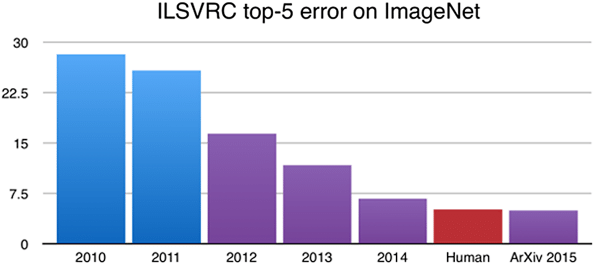
\includegraphics[width=7cm]{imnet_progress.png}}
%   \end{itemize}
% \end{frame}

% \begin{frame}
%   \frametitle{History : Revolution}
%   \begin{itemize}
%       \item<1->  1989 : Yann LeCun et al. refine backpropagation into the parallelisable form known today \cite{lecun1989backpropagation}
%       \item<2-> 1995 : Yann LeCun et al. invent Convolutional Neural Networks \cite{lecun1995convolutional}
%       \item<3-> 1998 : Yann LeCun et al. implement what has  become the industry standard for banks to recognize hand-written numbers on checks by training Convolutional Neurral Networks to classify zip codes from USPS data \cite{lecun1998gradient}. 
%       \item<4-> 2015 : Networks trained on Google's ImageNet database (>14M images, >20K categories) outperform humans \cite{SCHMIDHUBER201585}
%       \visible<4>{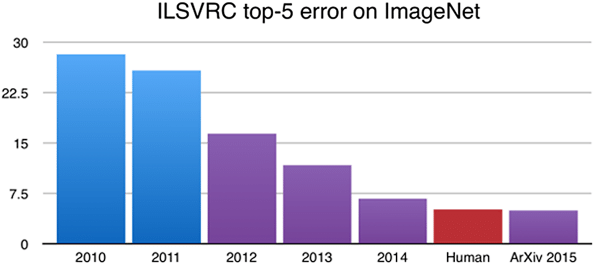
\includegraphics[width=7cm]{imnet_progress.png}}
%   \end{itemize}
% \end{frame}

% %%%%%%%%%%%%%%%%%%%%%%%%%%%%%%%%%%%%%%%%%%%(2) 

% \section{Introduction}
% % 1. define neural network input/output (neural style examples)
% %%%%%%%%%%%%%%%%%%%%%%%%%%%%%%%%%%%%%%%%%%%%%%%%%%%%%%%%%%%%%%%%
% \begin{frame}{Definitions}
% \begin{definition}{A \textbf{Neuron} is  }
%    a nonlinear operator that takes input in $\R^n$ to $\R$, historically designed to emulate the activation characteristics of an organic neuron.
%    \end{definition}
%    \begin{definition}{A}  
%     collection of neurons that are connected via a (usually directed) graph structure are known as an \emph{Artificial Neural Network (ANN)}.
%     \end{definition}
% \end{frame}

% \begin{frame}{Definitions}
% \begin{definition}{A \textbf{Perceptron} is  }
% \label{perceptron}
% a function $P_{\vec w}: \R^n \to \R$ which has \emph{weights} $\vec
% w \in \R^n$ corresponding with each element of an input vector $\vec
% x\in \R^n$ and a bias $b \in \R$:
% \[P_{\vec w}(\vec x) = f(\left(\ip{\vec w,\vec x} + b\right)\]
% \[P_{\vec w}(\vec x) = f\left(b + \sum_{i = 1}^n w_i x_i\right)\]
% where $f: \R \to \R$ is continuous. The function $f$ is called the \textbf{activation function} for $P$. 
% \end{definition}
    
% \end{frame}

% \begin{frame}{Definitions}
% \begin{definition}{The Rectified Linear Unit (ReLU) function is}
% \label{relu}

%   \[\relu(x) = \begin{cases} 0, & x \leq 0;\\
%       x, & x > 0,\end{cases}\]
% \end{definition}
% \begin{itemize}
%     \item ReLU works as well or better in most neural-network-type applications \cite{glorot2011deep}
% \item Training algorithms on ReLU activated networks converge faster \cite{nair_rectified_nodate}.
% \item The single nonlinearity at $x = 0$ is sufficient to guarantee $\epsilon$ approximation of smooth functions by an ANN composed of sufficiently numerous perceptrons connected by ReLU \cite{petersen2018optimal}. 
% \item ReLU is convex, which enables efficient numerical approximation of smooth functions in shallow networks  \cite{li2017convergence}.  
% \end{itemize}
% \end{frame}

% \begin{frame}{Definitions}
% \begin{definition}{Softmax (or the normalized exponential) is the function given by}
% \[s : \R^n \to [0,1]^n\]
% \[s_j(\vec x) = \frac{e^{x_j}}{\sum_{k = 1}^n e^{x_k}}\]
% \end{definition}

% \begin{definition}{We can define a classifier which picks the class corresponding with the largest output element from Softmax: }
% \[\text{(Output Classification)  }   c_s(\vec x) = \text{argmax}_{i} s_i(\vec{x})\]
% \end{definition}
    
% \end{frame}
% %%%%%%%%%%%%%%%%%%%%%%%%%%%%%%%%%%%%%%%%%(1)
% \begin{frame}{Training}
% What question are you trying to answer?
% 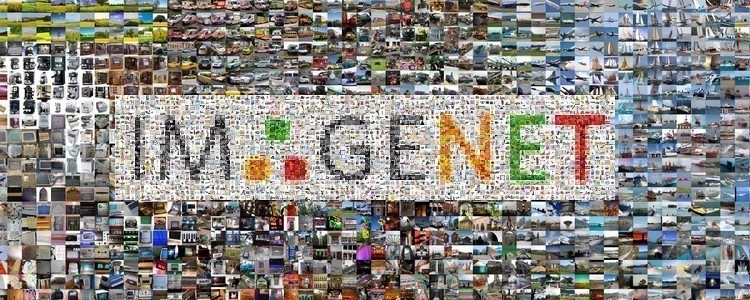
\includegraphics[width=7cm]{ImageNet-Title-Pic.jpg}

% 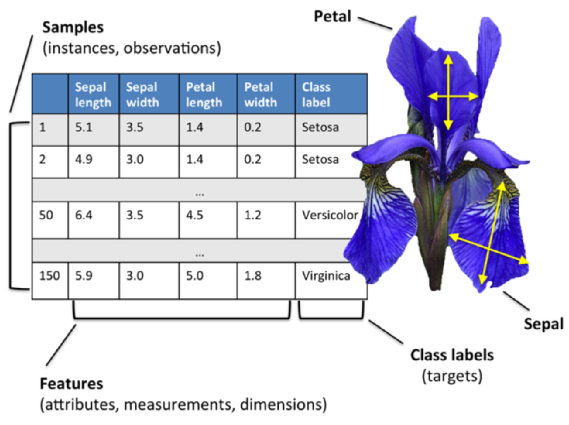
\includegraphics[width=5cm]{download (1).png}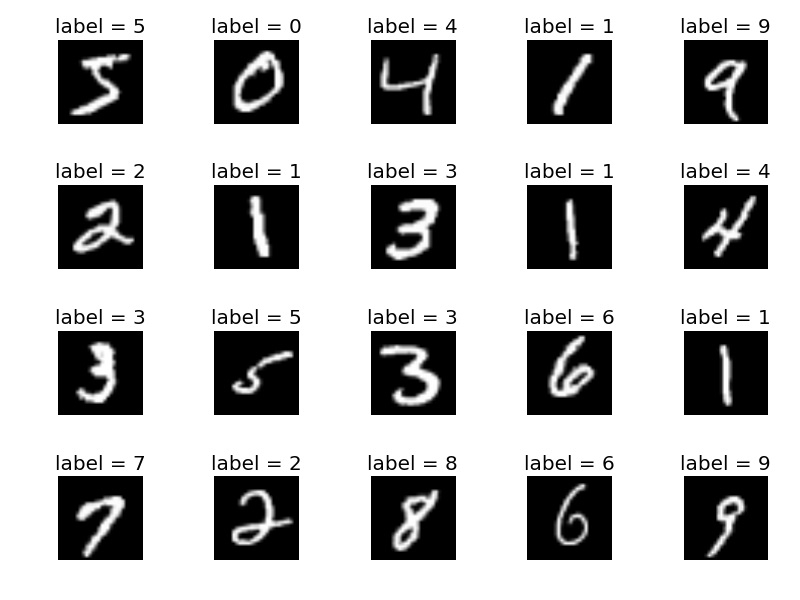
\includegraphics[width=5cm]{MNIST-dataset.jpg}
    
% \end{frame}
% \begin{frame}{Loss and Empirical Risk}
% \begin{definition}{The Cross-Entropy Loss comparing two possible outputs is}
% \[L(y,\hat y) = -\sum_i y_i \log \hat y_i\].
% \end{definition}

% \begin{definition}{Given a loss function $L$, the Empirical Risk over a training dataset $(X,Y)$ of size $N$ is }
% \[R_{\text{emp}}(P_{\vec w}(x) = \dfrac{1}{N} \sum_{(x,y) \in (X,Y)} L(P_{\vec w}(x)), y).\]
% \end{definition}
% We seek parameters $\vec w$ which will minimize $R_{\text{emp}}(P_{w}(x))$. This will be done with gradient-based optimization. 
    
% \end{frame}

% \begin{frame}{Computing Gradients}
   
% \scalebox{.9}{
% \begin{tikzpicture}[shorten >=1pt,->,draw=black!50, node distance=\layersep]

% \node[circle, minimum size=19pt, fill=black!25, inner sep=0pt] (n11) at (0,2) {$a^1_1$};
% \node[circle, minimum size=19pt, fill=black!25, inner sep=0pt] (n12) at (0,0) {$a^1_2$};
% \node[circle, minimum size=19pt, fill=black!25, inner sep=0pt] (n21) at (4,2) {$a^2_1$};
% \node[circle, minimum size=19pt, fill=black!25, inner sep=0pt] (n22) at (4,0) {$a^2_2$};
% \node[circle, minimum size=19pt, fill=black!25, inner sep=0pt] (n31) at (8,2) {$a^3_1$};
% \node[circle, minimum size=19pt, fill=black!25, inner sep=0pt] (n32) at (8,0) {$a^3_2$};

% \node (av1) at (0,2.9) {$\Bar{a}^1$};
% \node (av2) at (4,2.9) {$\Bar{a}^2$};
% \node (av3) at (8,2.9) {$\Bar{a}^3$};

% \node (ai1) at (0,3.9) {Index: $i$};
% \node (ai2) at (4,3.9) {Index: $\alpha$};
% \node (ai3) at (8,3.9) {Index: $\lambda$};

% \node (w2) at (2.6,2.9) {$W^2$};
% \node (w3) at (6.6,2.9) {$W^3$};


% \draw[- triangle 45] (n11)  -- node[rotate=0,shift={(0.3,0.3)}] {$w^2_{1,1}$} (n21);
% \draw[- triangle 45] (n11)  -- node[rotate=0,shift={(0.6,0.65)}] {$w^2_{1,2}$} (n22);
% \draw[- triangle 45] (n12)  -- node[rotate=0,shift={(0.3,-0.65)}] {$w^2_{2,1}$} (n21);
% \draw[- triangle 45] (n12)  -- node[rotate=0,shift={(0.6,-0.3)}] {$w^2_{2,2}$} (n22);

% \draw[- triangle 45] (n21)  -- node[rotate=0,shift={(0.3,0.3)}]  {$w^3_{1,1}$} (n31);
% \draw[- triangle 45] (n21)  -- node[rotate=0,shift={(0.6,0.65)}] {$w^3_{1,2}$} (n32);
% \draw[- triangle 45] (n22)  -- node[rotate=0,shift={(0.3,-0.65)}]  {$w^3_{2,1}$} (n31);
% \draw[- triangle 45] (n22)  -- node[rotate=0,shift={(0.6,-0.3)}]  {$w^3_{2,2}$} (n32);
% \end{tikzpicture}
% }

% \only<1>{ Terms will be indexed as follows:
% \[ x^{\text{[layer]}}_{\text{[node in layer], [node in previous layer]}}\]
% When the second subscript is omitted, the subscript will only index the node in the current layer to which this element belongs.}
% \only<2>{We can now write the output $\bar a_n$ for any layer of an arbitrary ANN in two ways \cite{Krause20}. Recursively, we can define
% \begin{equation}
%     a^n_\lambda = A^n(\sum_\alpha w^n_{\alpha, \lambda} a^{n-1}_\alpha)
% \end{equation}}

% \only<3>{We can also write the matrix form of this recursion for every node in the layer:
% \begin{equation}
% \bar a^n = \bar A^n (W^n(\bar a^{n-1} ) )
% \end{equation}}

% \only<4>{The matrix form makes it easier to write out a closed form for the output of the neural network. 
% \begin{equation}
% \bar a^n = \bar A^n (W^n(\bar A^{n-1}( W^{n-1} ( \cdots ( \bar A^{2} ( W^{2} \bar a^1) ) \cdots ) ) ) )
% \end{equation}}

% \only<5>{Now, given a loss function $L = \sum_{i} \ell_i(a^n_i)$ where each $\ell_i$ is a loss function on the $i^{\text{th}}$ element of the output, we wish to compute the derivatives $\dfrac{\partial L}{\partial_{w^l_{i,j}}}$ for every $l, i,$ and $j$ which compose the gradient $\nabla L$.}

% \only<6>{Using the diagram above, we can compute this directly for each weight using chain rule:
% \begin{align*}
%     \dfrac{\partial L}{\partial w^3_{\lambda,\alpha}} &= \dfrac{\partial L}{\partial a^3_{\lambda}} \dfrac{\partial a^3_{\lambda}}{\partial w^3_{\lambda,\alpha}} = \sum_{\lambda=1}^n \ell'_\lambda( a^3_\lambda) A'^3 (\sum_{\alpha=1}^n w^3_{\alpha, \lambda} a_\alpha^2) a^2_\alpha\\    
%     %\dfrac{\partial L}{\partial w^2_{\alpha,i} } &= \sum_{\lambda} \dfrac{\partial L}{\partial a^3_{\lambda}} \dfrac{\partial a^3_{\lambda} }{\partial w^3_{\lambda,\alpha}} \dfrac{\partial a^2_\alpha }{ w^2_{\alpha,i}}\\
% \end{align*}}


% \only<7>{Notice that $\ell'_\lambda$ and $A'^n$ are well understood functions 
% whose derivatives can be computed analytically almost everywhere. We can see that all of the partials will be of the form 
% $\dfrac{\partial L}{\partial w^l_{n, i}} = \delta^l_n a^l_i$ where $\delta^l_n$  will contain terms which are either pre-computed or can be computed analytically.}

% \only<8>{Conveniently, we can define this error signal recursively: 
% \[
% \delta^l_n = A'^l (a^l_{n}) \sum_{i = 1}^n w^{l+1}_{i, n} \delta^{l+1}_i
% \]
% In matrix form, we have
% \[\bar \delta^l = \bar A'^l(W^l \bar a^l) \odot ((W^{l+1})^T \bar \delta^{l+1}\]
% Where $\odot$ signifies element-wise multiplication. }

% \only<9>{Then we can compute the gradient with respect to each layer's matrix $W^l$ as an outer product: 
% \[\nabla_{W^l} L = \bar \delta^l \bar a^{(l-1)T}\]
% Since this recursion for layer $n$ only requires information from layer $n+1$, this allows us to propagate the error signals that we compute backwards through the network.}
% \end{frame}

% \begin{frame}{Optimizing Weights}
%     We can start with some
% default arrangement of the weights and choose a step
% size $\eta$ for gradient descent. Then for each weight, in each iteration
% of the learning algorithm, we apply a correction so that 
% \[w'_{i',j',k'} = w_{i',j',k'}-\eta \frac{\partial E(Y,\hat Y)}{\partial
%     w_{i',j',k'}}\]
    
%     However, ANNs lack guarantees for global convexity  \cite{Bishop:2006:PRM:1162264}, so this method often converges poorly or not at all. 
% \end{frame}

% \begin{frame}{Optimizing Weights}
% \begin{definition}{Stochastic Gradient Descent (SGD)}

% Given an ANN $N: \R^n \to C$, an initial set of weights for this network $\vec w_0$ (usually a small random perturbation from 0), a set of training data $X$ with labels $Y$, and a learning rate $\eta$, the algorithm is as follows: 

% \begin{algorithm}[H]
% \caption*{Batch Stochastic Gradient Descent}\label{sgd}
% \begin{algorithmic}[H]
% \State $w = w_0$
% \While{$E(\hat Y, P_w(X))$ (cumulative loss) is still improving} \Comment{ (the stopping condition may require that the weight change by less than $\e$ for some number of iterations or could be a fixed number of steps)}
% \State Randomly shuffle $(X,Y)$
% \State Draw a small batch $(\hat X, \hat Y) \subset (X, Y)$
% \State $w \leftarrow w - \eta \left(\sum_{(x,y) \in (\hat X, \hat Y)}  \nabla L(P_w(\hat x), \hat y)\right)$
% \EndWhile
% \end{algorithmic}
% \end{algorithm}
% \end{definition}
% \end{frame}
% %%%%%%%%%%%%%%%%%%%%%%%%%%%%%%%%%%%%%%%%%(1)
% \section{Adversarial Attacks}

% \begin{frame}
%   \frametitle{Intriguing Properties of Neural Networks \cite{Szegedy2013}}
% \begin{figure}[H]
%     \centering
% \includegraphics[width=5.5cm]{szegedy/negative1.png}\includegraphics[width=5.5cm]{szegedy/negative2.png}
%     \caption{Natural Images are in columns 1 and 4, Adversarial images are in columns 3 and 6, and the difference between them (magnified by a factor of 10) is in columns 2 and 5. All images in columns 3 and 6 are classified by AlexNet as "Ostrich" \cite{Szegedy2013}}
%     \label{fig:my_label}
% \end{figure}
% \end{frame}



% %%%%%%%%%%%%%%%%%%%%%%%%%%%%%%%%%%%%%%%%%%%(2)
% % 2. define classifier
% \begin{frame}
% \frametitle{Attacks : L-BFGS}
% Let $f : \R^m \to \{1,...,k\}$ be a classifier and assume $f$ has an associated continuous loss function denoted by loss$_f : \R^m \times \{1,...,k\} \to \R^+$ and $l$ a target adversarial . \\
% \textbf{ Minimize} $\Norm{r}_2$ subject to:
% \begin{enumerate}[1.]
% \item $f(x + r) = l$
% \item $x + r \in [0,1]^m$
% \end{enumerate}

% The solution is approximated with L-BFGS as implemented in Pytorch or Keras. This technique yields examples that are close to their original counterparts in the $L^2$ sense.
% \end{frame}
% \begin{frame}{Attacks : L-BFGS : MNIST}
%     \begin{figure}[H]
% \label{lbfgsa}
% \includegraphics[trim=200 185 100 200, clip, width=6cm]{2019-04-10-adverse/mnist_examples/FC200-200-10-2448-O8-A0-attack_summary.png}\includegraphics[trim=200 185 100 200, clip,width=6cm]{2019-04-10-adverse/mnist_examples/FC200-200-10-2448-O8-A1-attack_summary.png}
% \includegraphics[trim=200 185 100 200, clip,width=6cm]{2019-04-10-adverse/mnist_examples/FC200-200-10-2448-O8-A2-attack_summary.png}\includegraphics[trim=200 185 100 200, clip,width=6cm]{2019-04-10-adverse/mnist_examples/FC200-200-10-2448-O8-A3-attack_summary.png}
% \includegraphics[trim=200 185 100 200, clip,width=6cm]{2019-04-10-adverse/mnist_examples/FC200-200-10-2448-O8-A4-attack_summary.png}\includegraphics[trim=200 185 100 200, clip,width=6cm]{2019-04-10-adverse/mnist_examples/FC200-200-10-2448-O8-A5-attack_summary.png}
% \caption{Original images on the left, Perturbation is in the middle, Adversarial Image (total of Original with Perturbation) is on the right. Column 1 shows an original 8 being perturbed to adversarial classes 0, 2, and 4. Column 2 shows adversarial classes 1, 3, and 5}
% \end{figure}
% \end{frame}
% \begin{frame}{Attacks : Distortion}
%     Borrowing a metric from Szegedy et al to compare the magnitude of these distortions, we will define
% \begin{definition}{Distortion is the $L^2$ norm of the difference between an original image and a perturbed image, divided by the square root of the number of pixels in the image: }
% \[\sqrt{\dfrac{\sum_i \hat (x_i - x_i)^2}{n}}\]
% \end{definition}
% Distortion is $L^2$ magnitude normalized by the square-root of the number of dimensions so that values can be compared for modeling problems with differing numbers of dimensions. 
% \end{frame}

% \begin{frame}{Attacks : L-BFGS : MNIST}
%     \begin{figure}[H]
% \label{lbfgsh}
% \includegraphics[trim=200 80 100 100, clip, width=12cm]{2019-04-10-adverse/mnist_examples/FC200-200-10-distortion_hist.png}
% \caption{A histogram of the distortion measured for each of 900 adversarial examples generated using L-BFGS against the FC-200-200-10 network on Mnist. Mean distortion is 0.089.}
% \end{figure}
% \end{frame}
% %%%%%%%%%%%%%%%%%%%%%%%%%%%%%%%%%%%%%%%%%%%%%%%%%%%%%%%(3)

% \begin{frame}{Attacks : L-BFGS : ImageNet}
%  \begin{figure}[H]
% \label{lbfgsis}
% \includegraphics[trim=200 185 100 200, clip, width=6cm]{2019-04-10-adverse/imnet_examples/vgg16-ILSVRC2012_val_00039098-O722-A965-attack_summary.png}\includegraphics[trim=200 185 100 200, clip, width=6cm]{2019-04-10-adverse/imnet_examples/vgg16-ILSVRC2012_val_00027142-O52-A347-attack_summary.png}
% \includegraphics[trim=200 185 100 200, clip, width=6cm]{2019-04-10-adverse/imnet_examples/vgg16-ILSVRC2012_val_00029901-O425-A468-attack_summary.png}\includegraphics[trim=200 185 100 200, clip, width=6cm]{2019-04-10-adverse/imnet_examples/ILSVRC2012_val_00001375-Otensor([42])-A694-attack_summary.png}
% % \includegraphics[width=7cm]{2019-04-10-adverse/imnet_examples/vgg16-ILSVRC2012_val_00035978-O803-A353-attack_summary.png}
% % \includegraphics[width=7cm]{2019-04-10-adverse/imnet_examples/ILSVRC2012_val_00000886-Otensor([940])-A684-attack_summary.png}
% \caption{Original images on the left, Perturbation (magnified by a factor of 100) by is in the middle, Adversarial Image (total of Original with Perturbation) is on the right. Adversarial classes are Burrito, Bison, Taxi, and Paddle Wheel (Top Left, Top Right, Bottom Left, Bottom Right)}
% \end{figure}   
% \end{frame}

% \begin{frame}{Attacks : L-BFGS : ImageNet}
%     \begin{figure}[H]
% \label{lbfgsi}
% \includegraphics[trim=200 80 100 100, clip,width=12cm]{2019-04-10-adverse/imnet_examples/distortion_hist.png}
% \caption{A histogram of the distortion measured for each of 112 adversarial examples generated using L-BFGS against the VGG16 network on ImageNet images with mean distortion 0.0107}
% \end{figure}
% \end{frame}

% % 3. discuss solving neural networks, i.e. tuning weights. (gradient and
% %    back propagation passes error through the network)
% % 4. discus doing this computationally with torch or other
% %    multi-threading tools
% %%%%%%%%%%%%%%%%%%%%%%%%%%%%%%%%%%%%%%%%%%%%%%%%%%%%%%%%%%%%%%(2)
% \begin{frame}
% \frametitle{Attacks : FGSM}
% A single step attack process using the gradient of the loss function $L$ with respect to an image to find the adversarial perturbation \cite{goodfellow_explaining_2014}. for given $\e$, the modified image $\hat x$ is computed as
% \begin{equation}
% \hat{x} = x + \epsilon \text{sign} (\nabla L (P_w(x),x))
% \end{equation}

% This method is simpler and much faster to compute than the L-BFGS technique described above, but produces adversarial examples less reliably and with generally larger distortion.

% \end{frame}

% \begin{frame}
% \frametitle{Attacks : IGSM}
% In \cite{kurakin_adversarial_2016}
%   an iterative application of FGSM was proposed. After each
%   iteration, the image is clipped to a $\e L_\infty$ neighborhood of the original. Let $x'_0 = x$, then after $m$ iterations, the adversarial image obtained is:
% \begin{equation}
% x_{m+1}' = \text{Clip}_{x,\epsilon} \Bigl\{x_m' + \alpha \times \text{sign}(\nabla \ell (F(x'_m),x'_m))  \Bigr\} 
% \label{igsm}
% \end{equation}
% This method is faster than L-BFGS and more reliable than FGSM but still produces examples with greater distortion than L-BFGS. 
% \end{frame}

% \begin{frame}{Attacks : IGSM : ImageNet}
%     \begin{figure}[H]
%   \centering
% \includegraphics[trim=200 780 1200 212, clip,width=4cm]{2019-04-10-adverse/ILSVRC2012_val_00002900summary_plot.png}\includegraphics[trim=900 780 500 212, clip,width=4cm]{2019-04-10-adverse/ILSVRC2012_val_00002900summary_plot.png}
% %\includegraphics[width=12cm]{2019-04-10-adverse/ILSVRC2012_val_00048234summary_plot.png}
% \caption{adversarial example generated against VGG16 (ImageNet) with
% IGSM. Original Image (Rose Hip) on the left, adversarial image (Baseball) on the right. }
% \label{fgsmhip}
% \end{figure}
% \end{frame}
% %%%%%%%%%%%%%%%%%%%%%%%%%%%%%%%%%%%%%%%%%%%%%%%%%%%%%%%(3)
% \section{Stability Experiments}

% \begin{frame}{Classification Stability Under Perturbation}
%     \begin{definition}
% Consider a point $x \in X$ with corresponding class $c \in C$ and a classifier $\CC: X \to C$. We say that $x$ admits an \emph{$(\e,d)-$adversarial example} on $\CC$ if there exists a point $\hat x$ such that $d(x,\hat x) < \e$ and $\CC(\hat x) \neq c$. 
% \end{definition}
% This definition refers to the most general case of intentional mis-classification. The adversarial class can also be explicitly targeted:
% \begin{definition}
% Consider a point $x \in X$ with corresponding class $c \in C$ and a classifier $\CC: X \to C$. We say that $x$ admits an \emph{$(\e,d,c_t)-$targeted adversarial example} on $\CC$ if there exists a point $\hat x$ such that $d(x,\hat x) < \e$ and $\CC(\hat x) = c_t$. 
% \end{definition}
% \end{frame}

% \begin{frame}{Classification Stability Under Perturbation}

% \begin{definition}
% $x$ is \emph{$(\gamma,\sigma)$-stable} if $\mathbb{P}[\CC(x')=\CC(x)] \geq \gamma$ when $x' \sim \rho = N(X, \sigma^2 I)$ (i.e. $x'$ is drawn from a Gaussian with variance $\sigma$ and mean $x$).
% \end{definition}
    
% \end{frame}

% \begin{frame}{Classification Stability Under Perturbation}
%     We see that  
% \[\mathbb{P}[\CC(x')=\CC(x)] = \int \chi_{\CC^{-1}(\CC(x))} (x') d\rho (x') = \rho(\CC^{-1}\CC(x))\]
% In the case of images drawn from $\R^n$, we can write this integral precisely
% \[\dfrac{1}{\sigma(2\pi)^{n/2}} \int_{\R^n} \chi_{\CC^{-1}(\CC(x))} (y)e^{\dfrac{\norm{x - y}^2}{2\sigma^2}} d\vec y\]
% This integral is approximated by taking $N$ samples $x_k \sim \rho$ and computing 
% \[\dfrac{\norm{x_k : \CC(x_k) = \CC(x)}}{N}\]
% In our experiments, $\gamma$ is fixed and $\sigma$ is adjusted to determine the $\sigma$ for which an image is $\gamma-\sigma$ stable.
% \end{frame}

% \begin{frame}{Classification Stability Under Perturbation : MNIST}
%     \begin{figure}[H]
% \label{fgsmo}
% \includegraphics[trim=200 80 100 100, clip,width=12cm]{2019-04-10-adverse/Image918-O1Anone_varx40.png}
% \caption{Plotting frequency of each class in samples with increasing variance around natural image. Original Image Class is shown as a black curve. Bottom shows example sample images. }
% \end{figure}
% \end{frame}

% \begin{frame}{Classification Stability Under Perturbation : MNIST}
%     \begin{figure}[H]
% \label{fgsma}
% \includegraphics[trim=200 80 100 100, clip,width=12cm]{2019-04-10-adverse/Image918-O1A0_varx40.png}
% \caption{Plotting frequency of each class in samples with increasing variance around adversarial image. Adversarial class is shown as a red curve. Bottom shows example sample images. }
% \end{figure}
% \end{frame}

% \begin{frame}{Classification Stability Under Perturbation : MNIST}

% \begin{figure}[H]
% \includegraphics[trim=200 80 100 100, clip,width=12cm]{2019-04-10-adverse/original_hist.png}
% \caption{Histogram of $\sigma$ for $(\gamma=0.7, \sigma)$ stability of Adversarial Examples (Red) and Natural Examples (Blue)}
% \label{fgsmh}
% \end{figure}
% \end{frame}

% \begin{frame}{Classification Stability Under Perturbation : MNIST}
%     \begin{table}[H]

% \includegraphics[height=3.4cm]{Screenshot 2020-10-20 09.43.03.png}

% \begin{tabular}{|l|l|l|l|l|}
% \hline
% Network & Test Acc & Dist & Adv $(\gamma=0.7, \sigma)$ & Nat $(\gamma=0.7, \sigma)$ \\\hline
% FC10-4 & 92.09 & 0.123 & 1.68 & 0.93\\
% FC10-2 & 90.77 & 0.178 & 4.25 & 1.37\\
% FC10-0 & 86.89 & 0.278 & 12.22 & 1.92\\
% FC100-100-10 & 97.31 & 0.086 & 0.56 & 0.65\\
% FC200-200-10 & 97.61 & 0.087 & 0.56 & 0.73\\\hline
% \end{tabular}
% \caption{Recreation of Table 1 from Szegedy et al. using pytorch. New columns show $\sigma$ values which achieved $(\gamma=0.7,\sigma)$ stability for Adversarial and Natural examples. }
% \label{table1}
% \end{table}
% \end{frame}

% \begin{frame}{Classification Stability Under Perturbation : MNIST}
% \begin{figure}[H]
% \includegraphics[trim=200 80 100 100, clip,width=6cm]{2019-04-10-adverse/gamma_sigma/FC10-4-distortion_hist.png}\includegraphics[trim=200 80 100 100, clip,width=6cm]{2019-04-10-adverse/gamma_sigma/FC10-4-gamma1_hist.png}
% \caption{Distortion and $\sigma$ histograms for FC-10-4 in Table \ref{table1}}
% \label{table1hist1}
% \end{figure}
% \end{frame}

% \begin{frame}{Classification Stability Under Perturbation : MNIST}
% \begin{figure}[H]
% \includegraphics[trim=200 80 100 100, clip,width=6cm]{2019-04-10-adverse/gamma_sigma/FC10-2-distortion_hist.png}\includegraphics[trim=200 80 100 100, clip,width=6cm]{2019-04-10-adverse/gamma_sigma/FC10-2-gamma1_hist.png}
% \caption{Distortion and $\sigma$ histograms for FC10-2 in Table \ref{table1}}
% \label{table1hist2}
% \end{figure}
% \end{frame}

% \begin{frame}{Classification Stability Under Perturbation : MNIST}
% \begin{figure}[H]
% \includegraphics[trim=200 80 100 100, clip,width=6cm]{2019-04-10-adverse/gamma_sigma/FC10-0-distortion_hist.png}\includegraphics[trim=200 80 100 100, clip,width=6cm]{2019-04-10-adverse/gamma_sigma/FC10-0-gamma1_hist.png}
% \caption{Distortion and $\sigma$ histograms for FC10-0 in \ref{table1}}
% \label{table1hist3}
% \end{figure}
% \end{frame}

% \begin{frame}{Classification Stability Under Perturbation : MNIST}
% \begin{figure}[H]
% \includegraphics[trim=200 80 100 100, clip,width=6cm]{2019-04-10-adverse/gamma_sigma/FC100-100-10-distortion_hist.png}\includegraphics[trim=200 80 100 100, clip,width=6cm]{2019-04-10-adverse/gamma_sigma/FC100-100-10-gamma1_hist.png}
% \caption{Distortion and $\sigma$ histograms for FC100-100-10 in \ref{table1}}
% \label{table1hist4}
% \end{figure}
% \end{frame}

% \begin{frame}{Classification Stability Under Perturbation : MNIST}
% \begin{figure}[H]
% \includegraphics[trim=200 80 100 100, clip,width=6cm]{2019-04-10-adverse/gamma_sigma/FC200-200-10-distortion_hist.png}\includegraphics[trim=200 80 100 100, clip,width=6cm]{2019-04-10-adverse/gamma_sigma/FC200-200-10-gamma1_hist.png}
% \caption{Distortion and $\sigma$ histograms for FC200-200-10 in \ref{table1}}
% \label{table1hist5}
% \end{figure}
% \end{frame}

% \begin{frame}{Classification Stability Under Perturbation : ImageNet}
% \begin{figure}[H]
% \includegraphics[width=12cm]{2019-04-10-adverse/50r1000x_cmap_rand.png}
% \caption{Top heatmap indicates Gaussian samples added to a pure black image,\\
% Middle heatmap indicates Gaussian samples added to $x$ (the original image),\\
% Bottom heatmap indicates Gaussian samples added to $x + x_a$ (the adversarial image).}
% \label{imnetheat}
% \end{figure}
% \end{frame}

% \section{Future Work}

% \begin{frame}{Future Work}
% \begin{itemize}
%     \item Collect more data on stability for networks of varying complexity. 
%     \item Expand stability experiments on ImageNet
%     \item Use more sophisticated distributions to sample neighborhoods around examples. 
%     \item Generate adversarial examples which match natural images in stability and analyze distortion
%     \item Apply Bayesian Neural Network training techniques (and code) to refine distributional sampling. 
    
% \end{itemize}
    
% \end{frame}

% % \begin{frame}
% % \frametitle{Back-Propagation}
% % \begin{align*}
% % \frac{\partial E(Y,\tilde Y)}{\partial{w_{i',j',k'}}} &=  \frac{1}{2 N m_n}
% %   \sum_{\tilde y \in \tilde Y} a_{\tilde y}\sum_{j = 1}^n  \frac{\partial (
% %   \tilde y_j -
% %     y_j)^2}{\partial w_{i',j',k'}}\\
% % \frac{\partial (\tilde y_j - y_j)^2}{2 \partial w_{i',j',k'}} &= 
% % (\tilde y_j - y_j) \frac{\partial y_j}{\partial w_{i',j',k'}}
% % \end{align*}
% % Chain Rule Many (Many) Times:
% % \begin{align*}
% % (\tilde y_j - y_j) \frac{\partial y_j}{\partial w_{n,j',k'}} &= 
% % (\tilde y_j - y_j) \frac{\partial g_n\left(b_{n,j} + \sum_{k = 1}^{M_{n
% %                                                              - 1}} 
% % w_{n,j',k} O_{n - 1,k} \right)}{\partial w_{n,j',k'}}\\
% % &= 
% % (\tilde y_j - y_j)  g'_n\left(b_{n,j} + 
% % \sum_{k = 1}^{M_{n - 1}}w_{n,j',k} O_{n - 1,k} \right) O_{n - 1,k'}\\ 
% % \end{align*}

% % \cite{Bishop:2006:PRM:1162264}
% % \end{frame}

% % \begin{frame}
% % \frametitle{Back-Propagation}
% % We will collect
% % the other terms into a new term, 
% % \begin{align*}
% % \Delta_{n,j} &= (\tilde y_j - y_j)  g'_n\left(b_{n,j} + 
% % \sum_{k = 1}^{M_{n - 1}}w_{n,j',k} O_{n - 1,k} \right)\\
% % \Delta_{i,j} &= g'_n\left(b_{i,j} + 
% % \sum_{k = 1}^{M_{i - 1}}w_{i,j',k} O_{i - 1,k} \right)\sum_{k =
% %                1}^{m_{i+1}}w_{i+1,j,k} \Delta_{i+1,j}\\
% % \end{align*}
% % Thus the derivative we seek will be of the form
% % \begin{align*}
% % \frac{\partial (\tilde y_j - y_j)^2}{2 \partial w_{i',j',k'}} &=
% %   \Delta_{i,j} O_{i - 1,k'}\\
% % \end{align*}
% % \end{frame}


% % show the pictures generated
% %%%%%%%%%%%%%%%%%%%%%%%%%%%%%%%%%%%%%%%%%(1)

% %\begin{frame}
% %  \frametitle{Training}
% %
% %\end{frame}

% % \begin{frame}
% %   \frametitle{Training}
% % \begin{figure}
% %     \includegraphics[width=10cm]{2018-12-10-adverse/03-hw23_0-1_learn_mk-100.png}
% % \end{figure}
% % \end{frame}

% % \begin{frame}[fragile]
% % \frametitle{Training}
% % \begin{small}
% % \begin{verbatim}
% % class Net(nn.Module):
% %     def __init__(self, conf):
% %         super(Net, self).__init__()
% % 		# layers
% %         pairs = zip(conf[:-1], conf[1:])
% %         self.fcs = nn.ModuleList(nn.Linear(this_layer, next_layer)
% %                        for (this_layer, next_layer) in pairs)
% %     def forward(self, x):
% % 		# activation
% %         for layer in self.fcs[:-1]:
% %         x = F.relu(layer(x))
% %         x = self.fcs[-1](x)
% %         return x

% % conf = [28*28, 100, 25, 10]
% % \end{verbatim}n
% % \end{small}
% % 97.9\% accuracy on Mnist with 1000 epochs of training. 
% % \end{frame}

% % \begin{frame}{Complex Tasks}
% % \begin{figure}[h!]
% % \centering    
% % \movie[label=show3,width=1.0\textwidth,poster
% %        ,autostart,showcontrols,loop] 
% %   {}{arz1-big-white-16-compressed.mp4}
% %   \caption{caption}
% %  \end{figure} 
% % \end{frame}

% %\begin{frame}[fragile]
% %\frametitle{Performance}
% %\small
% %\begin{tabular}{l|l|l|l|l|l|l|l}
% %Model & Top-1 & Top-5 & Ops & GPU & CPU & Cfg & Weights  %\\\hline
% %AlexNet & 57.0 & 80.3 & 2.27 Bn & 3.1 ms & 0.29 s & cfg & 238 %MB\\
% %Darknet Reference & 61.1 & 83.0 & 0.96 Bn & 2.9 ms & 0.14 s & %cfg & 28 MB\\
% %VGG-16 & 70.5 & 90.0 & 30.94 Bn & 9.4 ms & 4.36 s & cfg & 528 %MB\\
% %Extraction & 72.5 & 90.8 & 8.52 Bn & 4.8 ms & 0.97 s & cfg &% 90 MB\\
% %Darknet19 & 72.9 & 91.2 & 7.29 Bn & 6.2 ms & 0.87 s & cfg & 80 MB\\
% %Darknet19 448x448 & 76.4 & 93.5 & 22.33 Bn & 11.0 ms & 2.96 s & cfg & 80 MB\\
% %Resnet 18 & 70.7 & 89.9 & 4.69 Bn & 4.6 ms & 0.57 s & cfg & 44 MB\\
% %Resnet 34 & 72.4 & 91.1 & 9.52 Bn & 7.1 ms & 1.11 s & cfg & 83 MB\\
% %Resnet 50 & 75.8 & 92.9 & 9.74 Bn & 11.4 ms & 1.13 s & cfg & 87 MB\\
% %Resnet 101 & 77.1 & 93.7 & 19.70 Bn & 20.0 ms & 2.23 s & cfg & 160 MB\\
% %Resnet 152 & 77.6 & 93.8 & 29.39 Bn & 28.6 ms & 3.31 s & cfg & 220 MB\\
% %ResNeXt 50 & 77.8 & 94.2 & 10.11 Bn & 24.2 ms & 1.20 s & cfg & 220 MB\\
% %ResNeXt 101 (32x4d) & 77.7 & 94.1 & 18.92 Bn & 58.7 ms & 2.24 s & cfg & 159 MB\\
% %ResNeXt 152 (32x4d) & 77.6 & 94.1 & 28.20 Bn & 73.8 ms & 3.31 s & cfg & 217 MB\\
% %Densenet 201 & 77.0 & 93.7 & 10.85 Bn & 32.6 ms & 1.38 s & cfg & 66 MB\\
% %Darknet53 & 77.2 & 93.8 & 18.57 Bn & 13.7 ms & 2.11 s & cfg & 159 MB\\
% %Darknet53 448x448 & 78.5 & 94.7 & 56.87 Bn & 26.3 ms & 7.21 s & cfg & 159 MB\\
% %\end{tabular}
% %Summary stolen from \cite{mohammad16}
% %\end{frame}



% %%%%%%%%%%%%%%%%%%%%%%%%%%%%%%%%%%%%%%%%%%%(2)













%\input{BeamerIntro.tex}
%\input{BeamerOverlays.tex}
%\input{funmath.tex}
%\input{BeamerConcl.tex}
\begin{frame}[allowframebreaks]
\frametitle{Citations}
\small{
\bibliographystyle{apalike}
%\bibliography{"\string~/Google Drive/dropbox/Dropbox/UOFA/0-research/bibfile"}
%\bibliography{'../bibfile'}{}
\bibliography{example}
}
\end{frame}


\end{document}


% TODO add in the papers from this semester for Thursday